% Select one class
%\documentclass{pucthesis}		% For DVI
\documentclass[pdftex]{pucthesis}	% For pdfLaTeX
%\documentclass[spanish]{pucthesis}		% For DVI, in spanish
%\documentclass[pdftex,spanish]{pucthesis}	% For pdfLaTeX, in spanish

%%%%%%%%%%%%%%%%%%%%%%%%%%
%      Nota: si usas español, algunos nombres      %
%      debes cambiarlos manualmente en este     %
%        documento. En teoría, nunca deberías       %
%           modificar el archivo pucthesis.cls              %
%%%%%%%%%%%%%%%%%%%%%%%%%%

%%%%%%%%%
%   Packages	 %
%%%%%%%%%
\usepackage{ textcomp }
% Floats
\usepackage{graphicx}
\usepackage{float}
\floatstyle{boxed}
\restylefloat{figure}
\usepackage{subfig}
\usepackage{color}

% Math packages
\usepackage{amsmath}
\usepackage{amsfonts}
\usepackage{amssymb}

% Closest font to Times New Roman
\usepackage{times}

% To make pretty tables
\usepackage{booktabs}
\usepackage{multirow}
\usepackage{pdflscape}


% To avoid underfull errors in the bibliography
\usepackage{etoolbox}
\apptocmd{\sloppy}{\hbadness 10000\relax}{}{}

% To make cites and references
\usepackage[hidelinks,pdfusetitle,pdfdisplaydoctitle]{hyperref}
\usepackage[notocbib]{apacite} 
\usepackage{doi}
\renewcommand{\doitext}{}

%--------- NEW ENVIRONMENTS --------- You are free to remove or use it
\newtheorem{definition}{\bf Definition}[chapter]
\newtheorem{property}{Property}[chapter]
\newtheorem{claim}{Claim}[chapter]
\newtheorem{lemma}{\bf Lemma}[chapter]
\newtheorem{proposition}{Proposition}[chapter]
\newtheorem{theorem}{\noindent \bf Theorem}[chapter]
\newtheorem{corollary}{\bf Corollary}[chapter]
\newtheorem{pf}{Proof}[chapter]
\newtheorem{example}{\bf Example}[chapter]
\newtheorem{remark}{Remark}[chapter]

\makeatletter
  \setlength{\beftitle}{105\p@\@plus24\p@}
  \setlength{\afttitle}{65\p@}
\makeatother

\begin{document}

\mdate{July 30, 2020}         % date manuscript changed
\version{1}                                     % manuscript version #

\title[Deep Neural Network Models with explainable components for urban space perception.]
   {\bf Deep Neural Network Models with explainable components for urban space perception.}       
\author[Andrés Cádiz Vidal]{Andrés Cádiz Vidal}

\address{Escuela de Ingenier\'ia\\
                   Pontificia Universidad Cat\'olica de Chile\\ 
                   Vicu\~na Mackenna 4860\\
                  Santiago, Chile\\
                  {\it Tel.\/} : 56 (2) 354-2000}
\email{username@uc.cl}

\facultyto    {the School of Engineering}
%\department   {}
\faculty                             {Faculty of Engineering}
\degree                  {Master of Science in Engineering}  %   {Mag\'ister en Ciencias de la Ingenier\'ia}  %        
                                 % or {Doctor in Engineering Sciences}    % {Doctor en Ciencias de la Ingenier\'ia}
\advisor                            {Hans Löbel}
\committeememberA {Patricio de la Cuadra}
\guestmemberA            {Member B}
\ogrsmember                 {Member C}
\subject                            {Structural Engineering}
\date                                 {July 2020}
\copyrightname             {Andrés Cádiz Vidal}
\copyrightyear               {MMXX}
\dedication                      {Gratefully to my parents and siblings}

%%%%%%%%%%%%%%%%%%%%
%       PRELIMINARIES                              %
%----------------------------------------------------%
%      page i & ii: cover page                   %
%      page iii: dedication                         %
%%%%%%%%%%%%%%%%%%%%

\NoChapterPageNumber
\pagenumbering{roman}
\maketitle

%%%%%%%%%%%%%%%%%%%%
%   EXTRA PAGES                                     %
%----------------------------------------------------%
%      page --: not used                             %
%%%%%%%%%%%%%%%%%%%%

%\newpage
%\thispagestyle{empty}

%----------------------------------------------------------------------%

%%%%%%%%%%%%%%%%%%%%%%%%%
%      page v: ACKNOWLEDGEMENTS                   %
%%%%%%%%%%%%%%%%%%%%%%%%%

\phantomsection \label{acknowledgements} % Comment if hyperref is unused
\chapter*{ACKNOWLEDGEMENTS}           
Thanks to my family and girlfriend for their unmeasurable support during the time
this research was done. Thanks to my advisor for his great guidance and contributions.
Thanks to all the members of \textit{IALAB PUC} and \textit{Instituto Milenio Fundamentos de los Datos}
project \#4 for all the very useful feedback and conversations. Thanks to ANID (former CONICYT) for
granting me the National Masters scholarship, which enabled me to complete my studies without
any issues.





\cleardoublepage

%----------------------------------------------------------------------%

%%%%%%%%%%%%%%%%%%
%          page v & up ---                      %
%            Table of contents              %
%            List of figures                     %
%            List of tables                      %
%%%%%%%%%%%%%%%%%%

\pdfbookmark{\contentsname}{toc}
\tableofcontents
\phantomsection \label{listoffigures}
\listoffigures
\phantomsection \label{listoftables}
\listoftables
\cleardoublepage

%----------------------------------------------------------------------%

%%%%%%%%%%%%%%%%%%%%%%%%
%      page x & xi: ABSTRACT - RESUMEN        %
%%%%%%%%%%%%%%%%%%%%%%%%

\phantomsection \label{abstract}
\chapter*{ABSTRACT}
Urban perception has been an important research subject for at least 60 years, with studies
being conducted by many different disciplines, using a variety of methodologies mainly based
on surveys over either real or simulated urban environments. The recently increased availability
of large amounts of data and highly scalable data collection methods powered by the modern web
has allowed for new techniques from other domains to be extended to the estimation of urban perception.
In particular, machine learning methods used as either stand alone models or feature extraction tools
have proven to be very effective for automatic quantification of the perception. This methods (neural networks in particular) present the disadvantage of having a black box
nature, which can make it hard for humans to understand the obtained results, therefore limiting
their application.

In this work we present a novel neural network architecture for automatic urban perception quantification.
Our best model, named AttnSegRank, can output an estimated urban perception score based on an image,
along with a set of weights (displayable as a heatmap) that reflect the importance of each part of the image
on the calculation of the score. It achieves this by including the output of a pretrained
semantic segmentator leveraged with an attention mechanism as part of the architecture. The model
we show in this work presents very similar performance with those in the previous literature but
with a much better interpretability, making it  not only a more useful model for urban perception
measuring and research, but a contribution to explainability in
the deep learning and computer vision fields that can be applied to other tasks as well.


\vfill
\noindent {\bf Keywords}:  urban perception, deep learning, explainable artificial intelligence.

\cleardoublepage

\phantomsection \label{resumen}
\chapter*{RESUMEN}
El resumen debe contener entre 100 y 300 palabras. El resumen debe ser escrito en ingl\'es y espa\~nol.  En el caso de tesis de doctorado, el formato de la p\'agina del resumen es distinta, por favor verifique la plantilla entregada por la Direcci\'on de Postrgrado.\

\vfill
\noindent {\bf Palabras Claves}: percepción urbana, aprendizaje profundo, inteligencia artificial explicable.

\cleardoublepage

%%%%%%%%%%%%%
%   TEXT  OF THESIS     %
%%%%%%%%%%%%%

\pagenumbering{arabic}

\chapter[INTRODUCTION]{Introduction}
\section{Thesis outline.}
\section{Importance of automatic urban perception}
\section{Importance of explainability in artificial intelligence}
\section{Hypothesis}

\chapter[RELATED WORK]{Related Work} \label{work}
This chapter consists of two sections, the first one shows an overview some of the
different methods that have been previously used in the literature
for understanding or estimating urban perception, these methods are separated
into 3 types: the classic approaches (all the methods not relying on
massive amounts of data are grouped here), approaches based on machine learning and
approaches consisting of machine learning models combined with other techniques.
The different methods are explained and a brief analysis of advantages and disadvantages
is provided for each of them. Section two summarizes the main aspects of the research
on explainability on deep learning, and describes some techniques that have been applied
in urban perception or other domains that are relevant for this work.


\section{Solutions for estimating urban perception.}

\subsection{Classic approaches.}
Methods for measuring perception of urban spaces have appeared in the literature of several
disciplines for many years,  with some of the most influential studies dating back to 1960
\cite{lynch}. Due to technological limits the literature consisted mainly of several types of
qualitative surveys for a long time. This surveys consisted in having subjects, complete
different tasks such as drawing maps of a certain place \cite{lynch}, evaluating fundamental
aspects of a neighborhood \cite{nasar_perception}, or in more recent approaches evaluating
the impact of transformations generated with edited images \cite{jiang_minimizing}. Most of
these surveys were conducted in person or by phone, and then the results were analyzed by hand.







\subsection{Pure machine learning approaches.}

\subsection{Mixed approaches.}

\section{ Explainability in deep learning.}

\chapter[DATASET]{Dataset} \label{dataset}
This chapter presents an analysis of the dataset used. On section \ref{sec:dataset_desc} an overall description
and main statistics are shown. Section \ref{sec:dataset_prep} presents an early analysis of the data along with
the preprocessing steps taken. Finally section 3 makes an analytical definition of the problem
of learning urban perception from this data.


\section{Description}
\label{sec:dataset_desc}
As was mentioned previously, this work is based on the Place Pulse 2.0 dataset \cite{hidalgo_placepulse}.
PP 2.0 is a crowdsourced dataset designed for learning urban perception from street view like images.
Unlike regular datasets for supervised machine learning, that have labels for each image, Place Pulse
consists of pairwise comparisons between images, and the ground truth is a vote representing which of
the images is more representative of an attribute (ties are also possible). That structure makes
traditional classification / regression approaches inapplicable, but opens the door for
pairwise based ranking techniques, that are more suitable to urban perception since a ground truth for
how much an image represents an abstract attribute such as "safety" it's impossible to define.

The dataset consists of approximately 1.2 million pairwise comparisons of 112,000 images from 56 cities,
distributed on 6 attributes: wealthy, safety, depressing, boring, lively and beautiful, making it
the biggest available dataset for urban perception. The crowdsourcing survey was
active for 5 years and it was answered by 81,630 different users. Demographic information
about the users was not collected.

\section{Analysis and preprocessing}
\label{sec:dataset_prep}

As a first preprocessing step all noisy images are removed by using a file size threshold,
since files small in size are mostly  google api errors or unintelligible places like
dark tunnels.

Is important to note that, unlike most crowdsourced datasets, the authors of PP did not
perform a validation on the votes. 99.59\% of the image pairs that appear in the
data set have a single vote in a category (see \ref{fig:rep_hist} for details.),
making it impossible to corroborate if they are reasonable by comparing the votes of multiple people.
Even though previous research indicates that answers to this surveys aren't affected by user
bias or demographics \cite{hidalgo_inequality, costa_lisbon}, the inconsistency in the votes is a
clear dataset disadvantage: 34\% of the  pairs that have more than one vote in an attribute
show inconsistencies between the votes.


\begin{figure}[ht]
	\begin{center}
	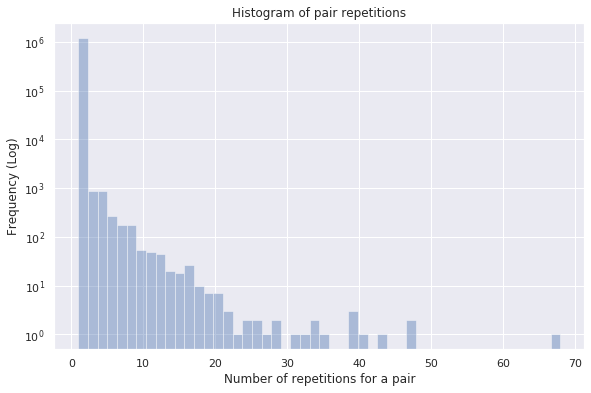
\includegraphics[width=0.8\textwidth]{./figures/rep_hist.png}
	\caption[Repetition histogram]{ Histogram for amount of repetitions for each pair of images }
	\label{fig:rep_hist}
	\end{center}
\end{figure}

For this work we completely remove all inconsistent duplicates and keep a single instance of those consistent.
After these, steps 1,207,938 votes for 111,299 images are left. See Table \ref{tab:votes}
for the exact vote distribution.

\begin{table}[H]
	\begin{center}
	\caption[Votes Distribution]{ Vote distribution after preprocessing.}
	\begin{tabular}{ll}
		\hline
		\textbf{Attribute} & \textbf{\# of votes} \\ \hline
		Wealthy            & 150,370               \\
		Safety             & 364,130               \\
		Depressing         & 130,781               \\
		Boring             & 125,744               \\
		Lively             & 263,123               \\
		Beautiful          & 173,790               \\ \hline
		Total              & 1,207,938            \\
	\end{tabular}
	\label{tab:votes}
	\end{center}
\end{table}

Users of the survey had the possibility of voting that a pair is tied for an attribute,
meaning that they didn't perceive any significant difference. Previous works usually
discard this data and don't use it for learning, focusing only on the votes where a preference was
chosen \cite{hidalgo_placepulse,zhang_measuring,tamara_judgments}. After preprocessing 15.3\% of the
votes are ties, which means a significant amount of information is lost by disregarding them.
Due to that we decided to add additional rules to the learning problem in order to be able to use
these votes for learning. Details are shown on the following chapter.

\chapter[PROPOSED MODEL]{Proposed Model} \label{arch}
This chapter presents a detailed explanation of the neural network models proposed in this work and
the correspondent baselines used for comparison. In Section \ref{sec:problem_def} we give a formal definition
of the learning problem. In Section \ref{sec:nn_arch} the architectures of
the main networks are shown. In Section \ref{sec:adds} we detailed additional components used on the models and training.
Finally, Section \ref{sec:baselines} shows the baselines models
used for the ablation study of both performance and explainability.


\section{Problem Definition}
\label{sec:problem_def}

Following a formulation similar to \citeA{hidalgo_placepulse}, each attribute $A$ in the PP 2.0
consists of a set $I_A$ of images and a set $P_A$ of votes for those images.
Each image in $I_A$ is a tensor $x \in \mathbb{R}^{h \times w \times 3}$ where $h$ and $w$ are the height and width respectively.
Each vote in $P_A$ is a triple $(x_1,x_2,y)$ where $x_1$ and $zx_2$ are images in $I_A$ and $y\in \{1,0,-1\}$.
A triple $(x_1,x_2,y)\in P_A$ represents a comparison where $y=1$ states a preference of $x_1$ over $x_2$, and $y=-1$
represents a preference of $x_2$ over $x_1$. The value $y=0$ represents a tie.

The objective is to, for each attribute, learn a ranking function $f_A : \mathbb{R}^{h \times w \times 3} \rightarrow \mathbb{R}$
that maps the image tensor to an urban perception score, satisfying the order given by the votes. Formally the
maximum amount of the following constraints need to be satisfied:

\begin{equation}
	y \cdot (f_A(x_1) - f_A(x_2)) > 0 \;  \forall (x_1,x_2,y) \in P_A\text{ and }y\in\{-1,1\}
	\label{eq:constraints}
\end{equation}

Unlike the previous literature, tie votes are also used in this work, generating the following additional constraints:

\begin{equation}
	|f_A(x_1) - f_A(x_2)| < m \;\; \forall (x_1,x_2,y) \in P_A\text{ and }y=0 \; ;  m \in \mathbb{R}^+
	\label{eq:constraints_ties}
\end{equation}

Where $m$ is a constant margin.

Since $f_A$ is intended to learn a ranking of the input images, it is desirable that the function defines an order
on the image space so that the ranking results are consistent. This condition can and should be enforced by
model design \cite{koppel_pairwise}, but since the data is crowdsourced without
validation, the constraints generated by equation \ref{eq:constraints}, do not represent a  100\% transitive order.
Because of that, it is infeasible for a model designed for ranking and therefore
transitive by construction, to satisfy all of them.
This issue makes it harder to obtain high scores in accuracy based metrics in practice, and
those are the only ones available in the literature so far.


\section{Network architectures}
\label{sec:nn_arch}
As was mentioned before, the main principle followed for model design is to enhance explainability
while maintaining performance of the model as much as possible. With that in mind, we combine two
state-of-the-art techniques from the deep learning literature, semantic segmentation
and attention mechanisms, to design three novel architectures that present a significant
improvement in explainability over traditional blackbox CNNs. We describe these architectures
in the following sub sections, ordered by model complexity. Is important to note that
for learning to rank on the Placepulse dataset,
two forward passes of the ranking  network are required for each data instance (one for each image) and both scores are used
for calculation of the loss. See section \ref{section:loss} for  details.


\subsection{SegRank base.}
The traditional deep learning approach in computer vision, consists of using a pretrained
CNN \cite{lecun_mnist}, on the Imagenet dataset \cite{imagenet}, such as the ResNet \cite{he_resnet},
usually called the feature extractor, and then stacking a custom set of layers over its output features. Leaving the CNN weights
fixed or updating them on training  depends on the particular problem. This is the approach taken
by most of the previous literature on urban perception \cite{hidalgo_placepulse,tamara_judgments,zhang_measuring}.

In this work, we propose replacing the traditional feature extractors for a fully trained semantic segmentation
network. The semantic segmentation task consists of assigning a label to every pixel in an image, and therefore
it implies a fine grained detection of object edges, providing a rich amount of information that is human understandable.
The output of a semantic segmentation model is a probability distribution over the different classes for each pixel,
making it usable as a feature map of the image. See Figure \ref{fig:segmentation} for an example.

We base our models on the PSPNet architecture \cite{pspnet}, since it is one of the highest performing models
available in the literature. It's design is based on a ResNet50 and a pyramid pooling module, which consists on
parallel poolings and convolutions at different scales, that are then concatenated and used to generate the output with a
final convolution.

\begin{figure}[ht]
	\begin{center}
	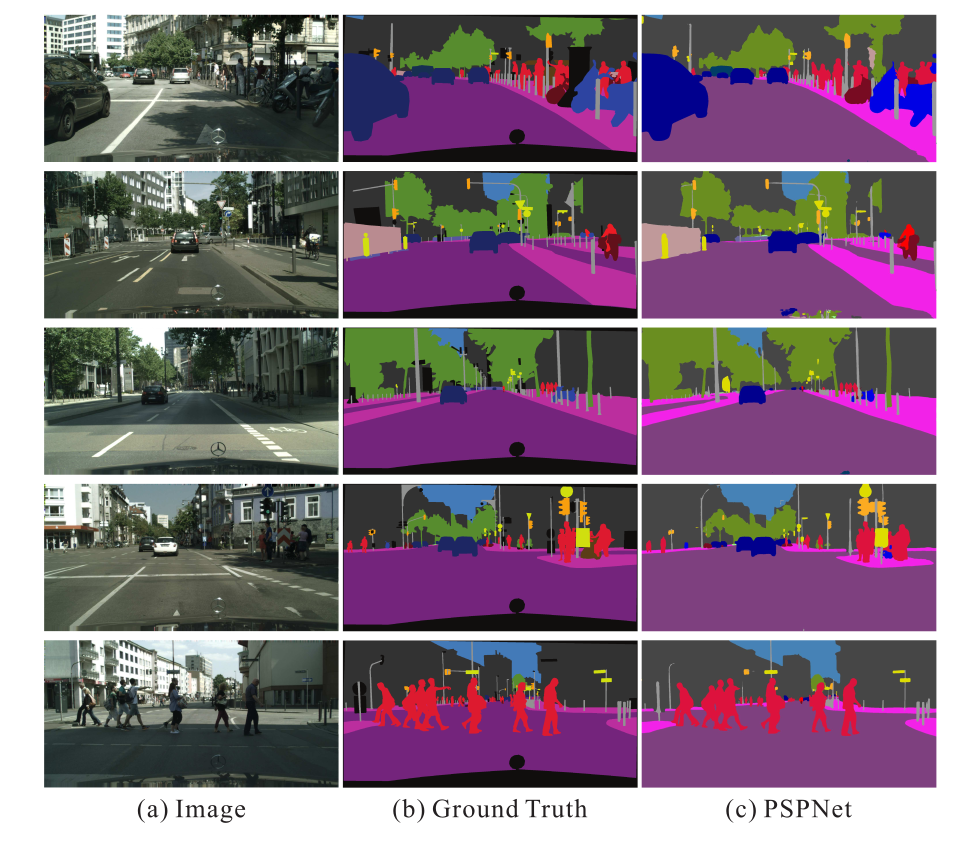
\includegraphics[width=0.8\textwidth]{./figures/segmentation.png}
	\caption[Example of Semantic Segmentation]{Examples of semantic segmentation by the PSPNet model on the CityScapes dataset. Extracted from \citeA{pspnet} }
	\label{fig:segmentation}
	\end{center}
\end{figure}

\begin{figure}[ht]
	\begin{center}
	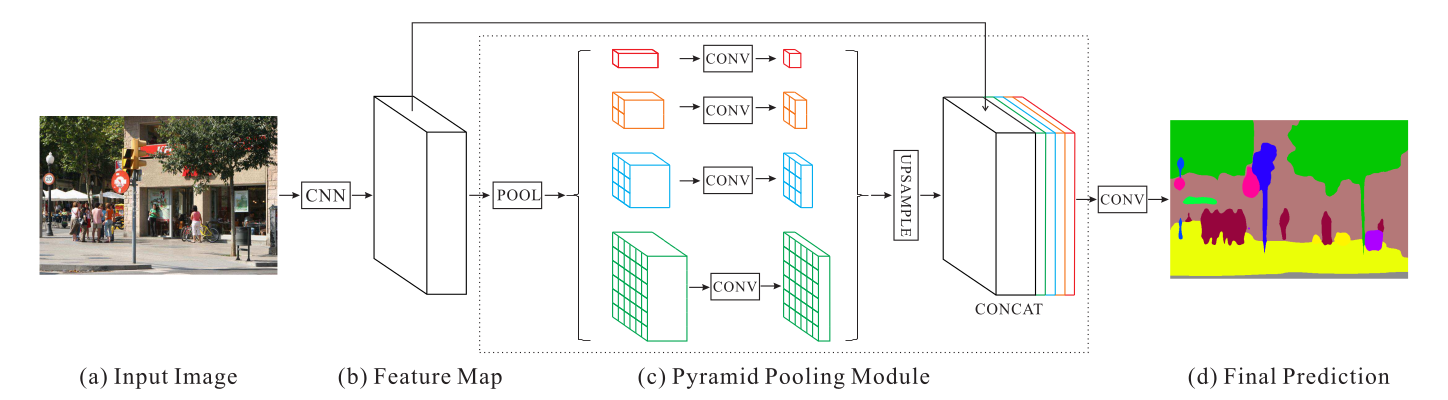
\includegraphics[width=0.9\textwidth]{./figures/pspnet.png}
	\caption[PSPNet architecture]{PSPNet architecture. Extracted from \citeA{pspnet} }
	\label{fig:segmentation}
	\end{center}
\end{figure}

We train PSPNet on the CityScapes dataset \cite{cordts_cityscapes}, since its urban images taken from a car have
considerable similarity to Street View images, and its classes have proven informative for the urban perception problem
in previous research \cite{rossetti,zhang_measuring}. After this process we keep the network weights fixed
and use the output as features for subsequent layers. The segmentation output  is a tensor $S$, $S \in \mathbb{R}^{h\times w \times C}$, with $C$
being the number of different classes. We experiment with using the features directly or applying a softmax operation.

For the calculation of the ranking score, we apply a linear transformation to every pixel distribution, flattening the output to
$\mathbb{R}^{h \times w}$  and then an MLP with one hidden layer and ReLU activation. The final linear layer
of the MLP generates a single scalar value representing the perception score.

It is important to note that the features given by  segmentation are  of considerable less dimensionality
than traditional ResNet features and only capture the very specific information of which class is each pixel,
which makes them  significantly less expressive. Adding to that,
since traditional CNN based approaches allow for finetuning, the amount of trainable parameters
is also much smaller for this model than traditional models. Due to these two reasons the learning capacity
of this model is much smaller, and therefore a significant performance drop is likely to happen.

\begin{figure}[ht]
	\begin{center}
	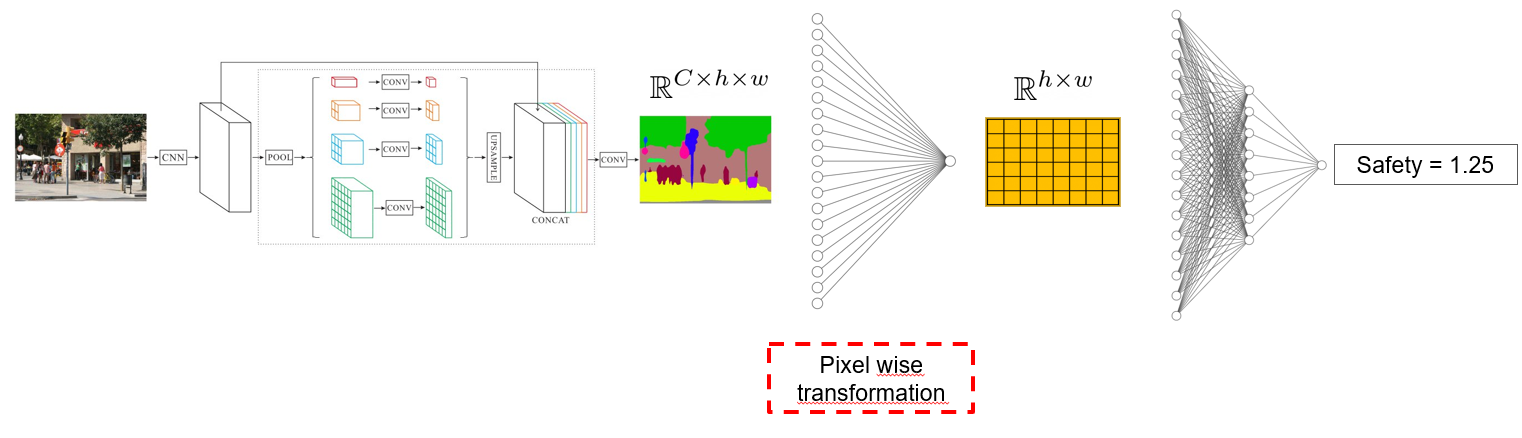
\includegraphics[width=0.9\textwidth]{./figures/segrank_1.png}
	\caption[First model architecture]{First model architecture}
	\label{fig:segrank_1}
	\end{center}
\end{figure}

\subsection{SelfSegRank}\label{section:self-attn}
With the intention of improving  performance and explainability of SegRankBase model, we process
the segmentation output with self attention mechanisms instead of a traditional MLP,
since it has been proven to provide benefits in both aspects by previous research \cite{vaswani_attention, wiegreffe_attention, cordonnier_relationship}.

For our model we use the scaled dot product attention mechanism
proposed by \citeA{vaswani_attention}. We abstain from using the full multi head attention
mechanism  that consists of the same operations but splitting the input in several ``heads''.
We do this because using multiple heads adds complexity to the interpretation of the attention outputs,
since different heads may output inconsistent weights, as is mentioned in \citeA{clark_bertlook}
and \citeA{li_disagreement} and also verified on this task by our own experiments.

The attention mechanisms receives three matrixes as input: the query $Q$, the key $K$ and the value
$V$. It calculates a matrix of attention weights over $V$ based on $Q$ and $K$ and the final output
is given by the product between $V$ and the weights. A linear transformation is defined
for each of the inputs with weights $W_Q, W_K, W_V$ respectively, and another transformation $W$
is applied to the final output (see Figure \ref{fig:attention_mech}).
Formally the attention layer can be defined as:
\begin{align}
	\label{eq:attention}
	\text{Attention}(Q,K,V) &= \text{softmax}\left (\frac{QK^T}{\sqrt{d_k}} \right ) V \\
	\label{eq:attention_layer}
	\text{AttentionLayer}(Q,K,V) &=  \text{Attention}(QW_Q,KW_K,VW_V)\cdot W
\end{align}
where $d_k$ is the embedding size of the key. For the particular case of self attention,
the same input is used as query, key and value, so for our case we make $Q=K=V=S'$ with
$S' \in \mathbb{R}^{(hw) \times C}$ and equal to the segmentation output flattened to one
spatial dimension.

\begin{figure}[ht]
	\begin{center}
	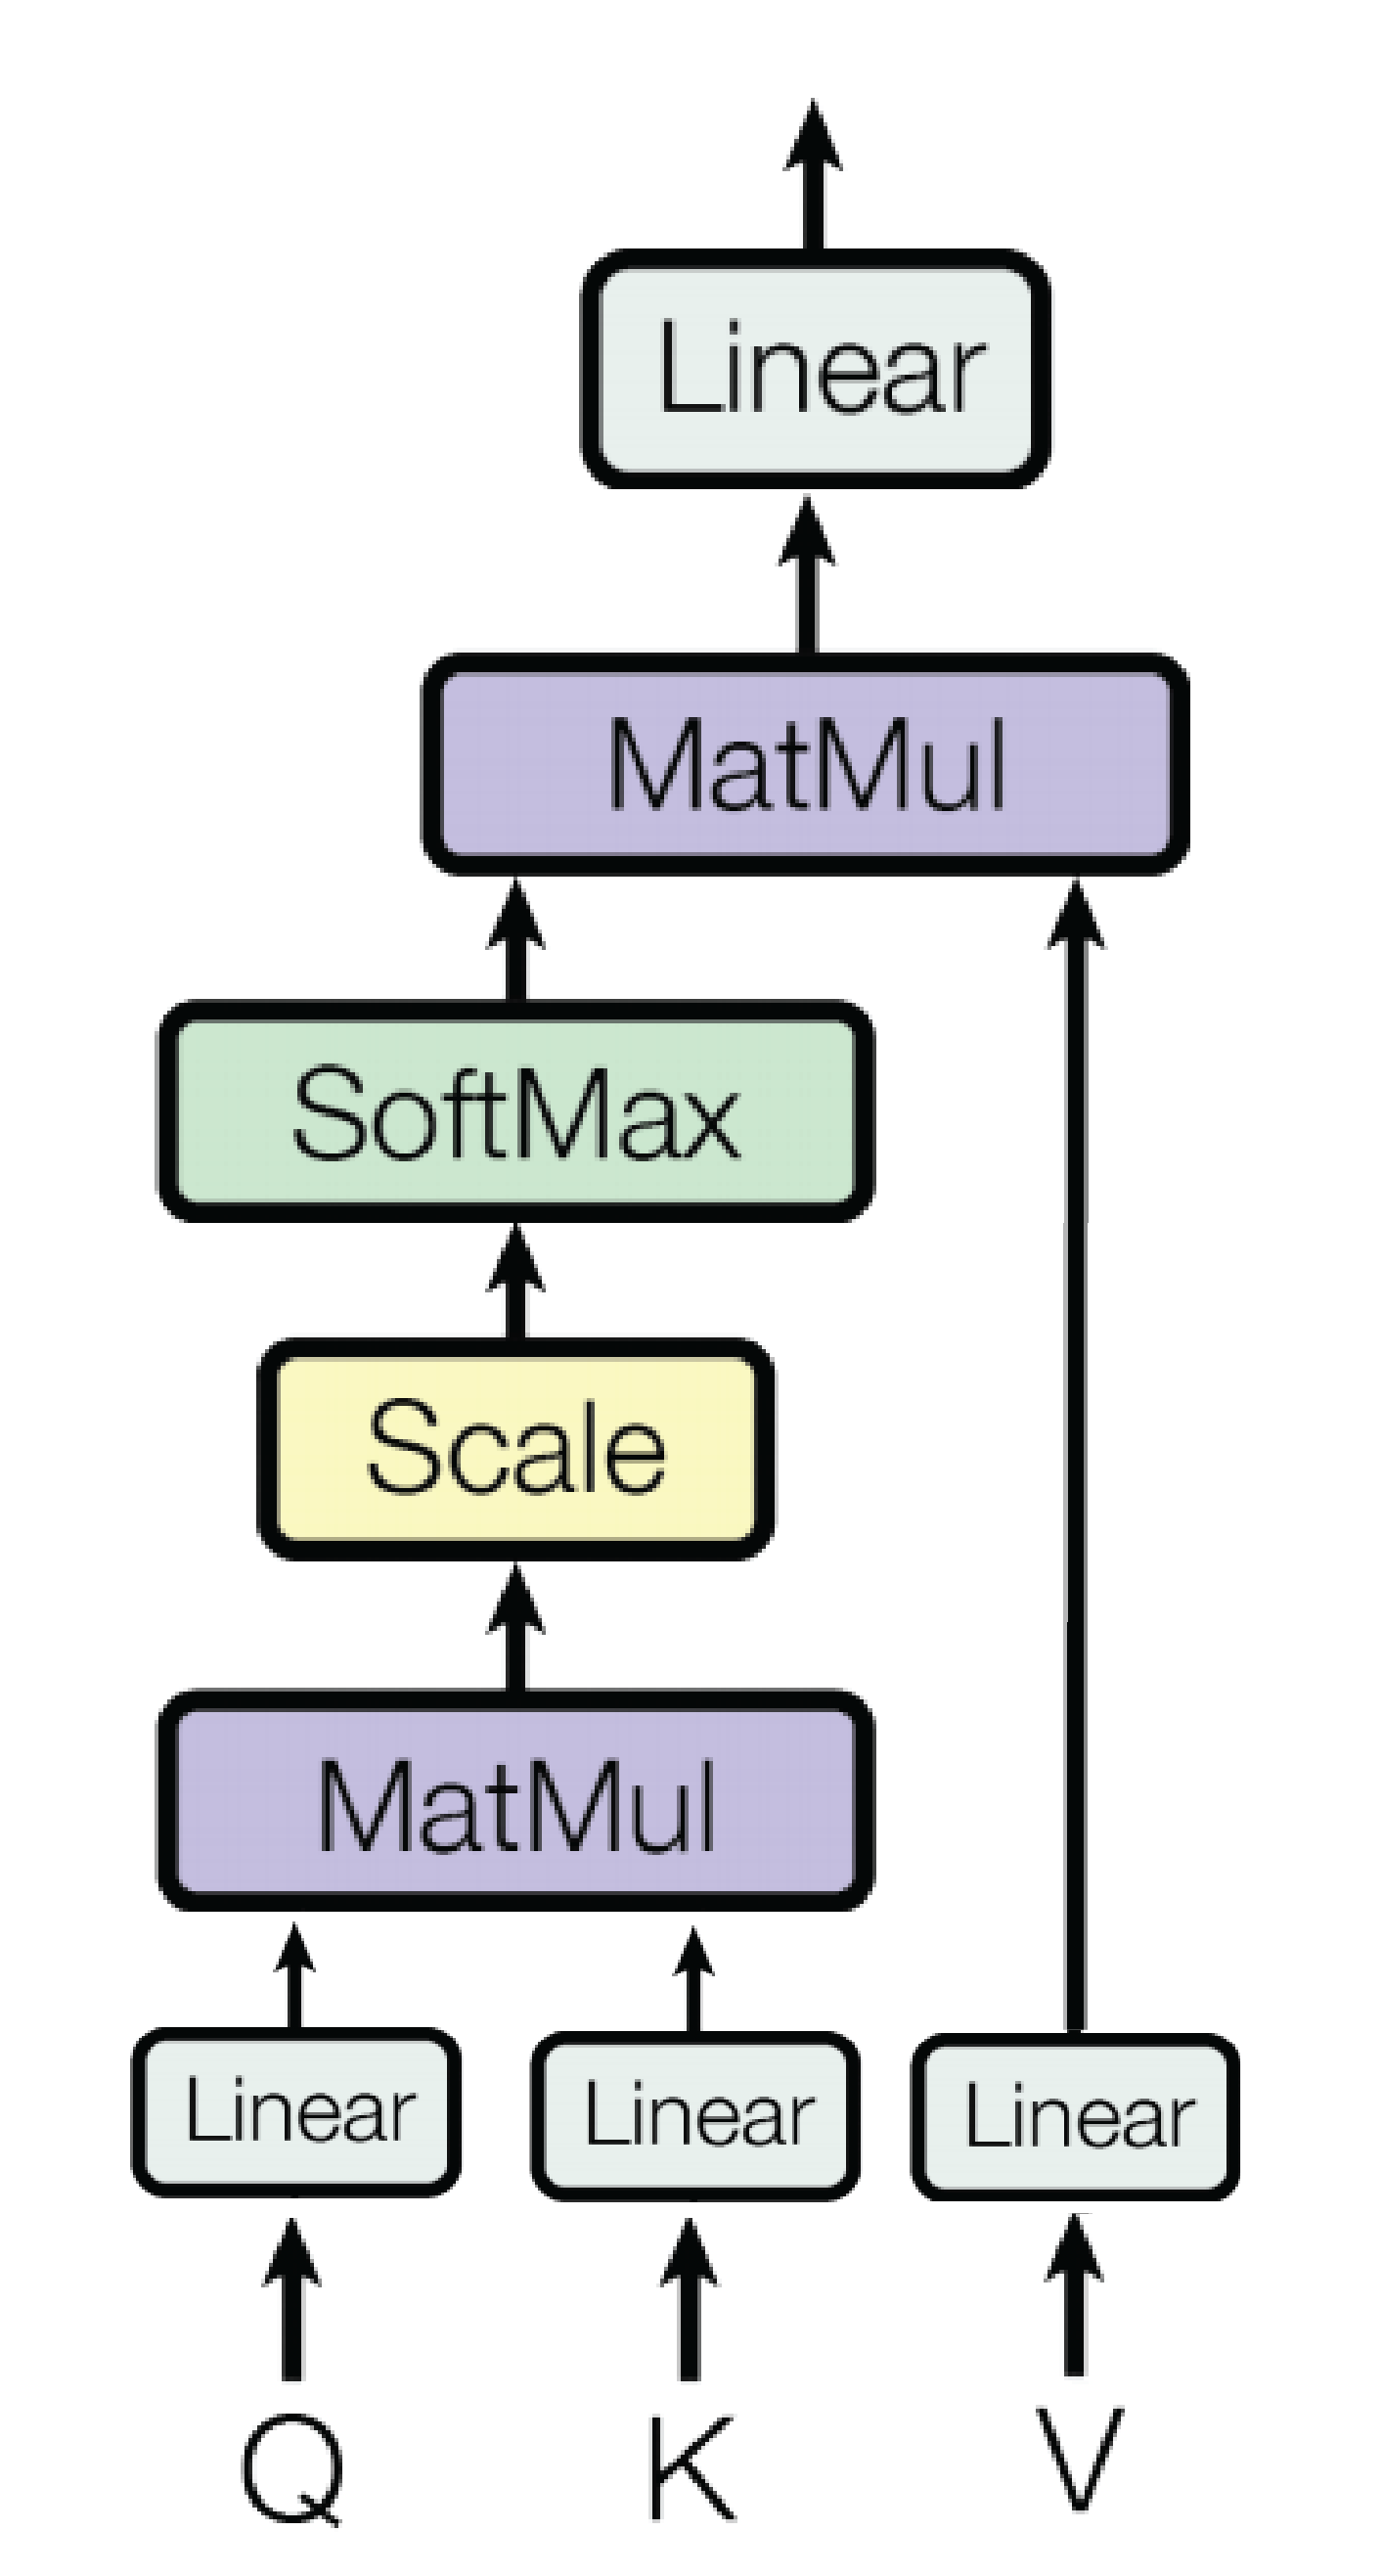
\includegraphics[width=0.3\textwidth]{./figures/attention.png}
	\caption[Attention Mechanism]{Attention layer operations. Adapted from \citeA{vaswani_attention}}
	\label{fig:attention_mech}
	\end{center}
\end{figure}

Similarly to the previous model, we apply a linear layer to calculate the ranking score from the attention output.
We only use one layer instead of two in this model because the attention mechanism already has a large amount of parameters and a
linear transformation of its own.
In parallel the attention weights are also outputted by the model and are used for visualization. Figure \ref{fig:selfsegrank}
shows a diagram of the full architecture

\begin{figure}[ht]
	\begin{center}
	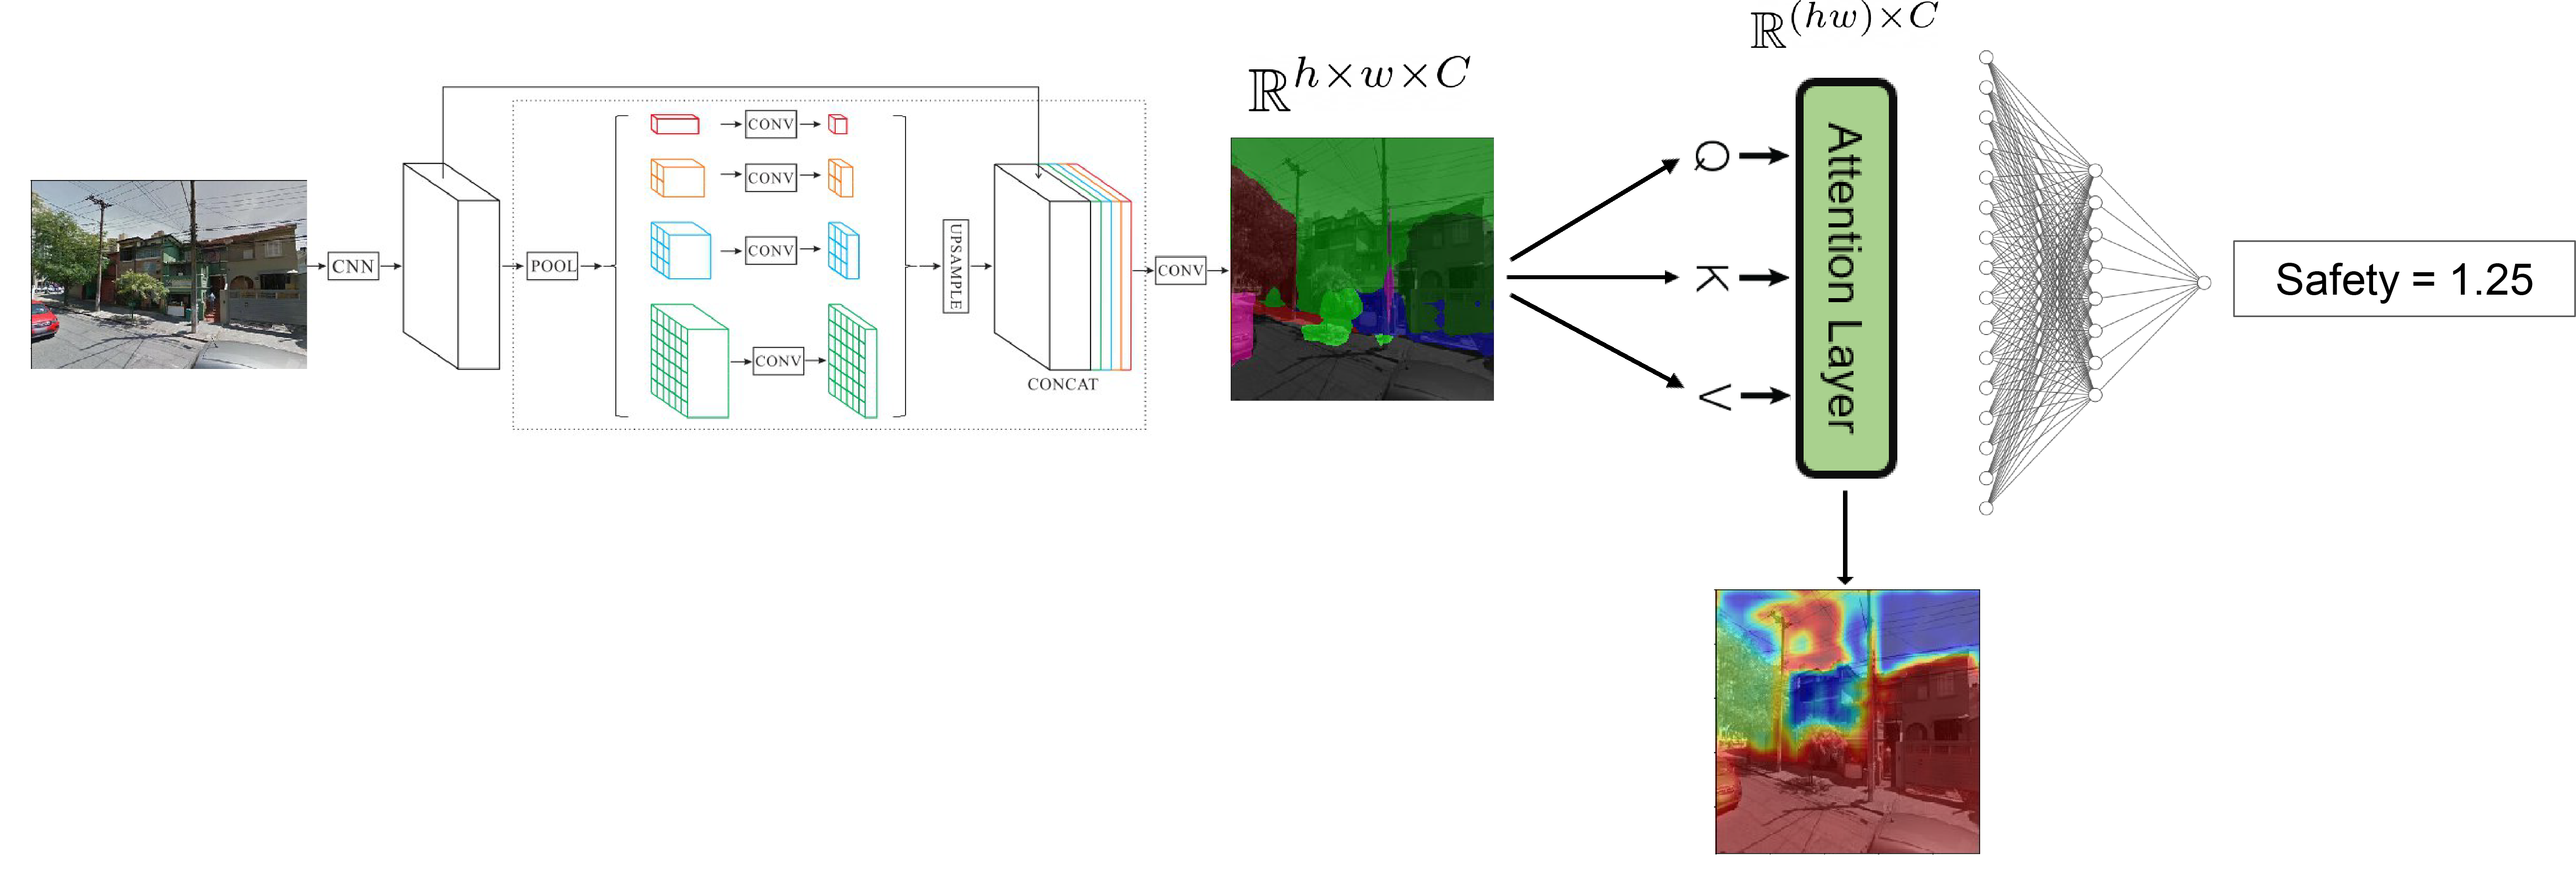
\includegraphics[width=1\textwidth]{./figures/self_attn.png}
	\caption[Self Attention network]{Segmentation and self attention network.}
	\label{fig:selfsegrank}
	\end{center}
\end{figure}

\begin{figure}[ht]
	\begin{center}
	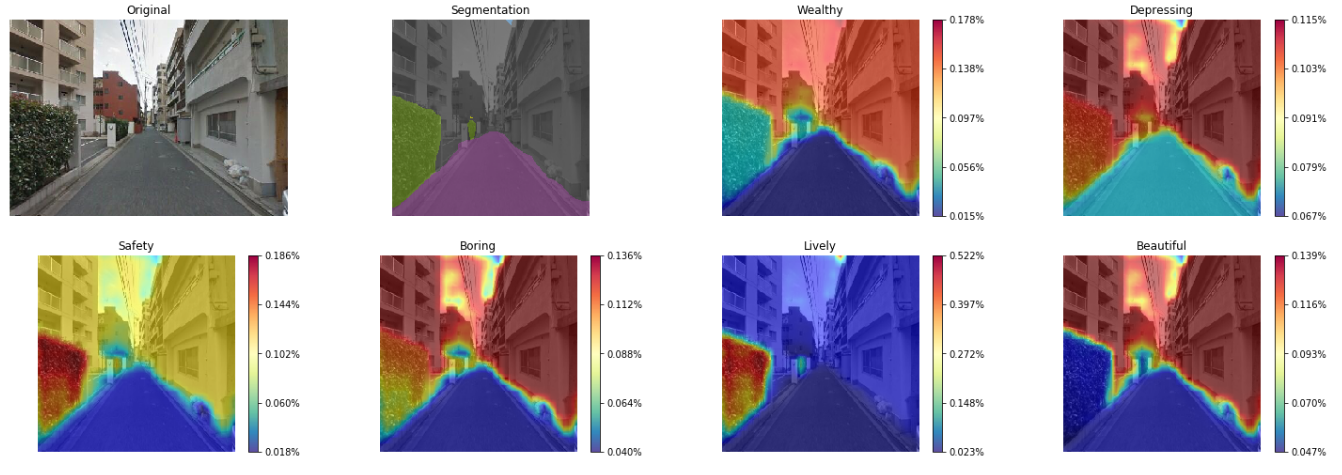
\includegraphics[width=1\textwidth]{./figures/self_attn_vis.png}
	\caption[Self Attention Model output]{Example segmentation and self attention weights for all six attributes.}
	\label{fig:segrank_attention}
	\end{center}
\end{figure}

As it can be seen on Figure \ref{fig:segrank_attention}, the attention weights keep the object shapes,
allowing for a clear interpretation of which objects are significant to the output.

\subsection{AttentionSegRank}
As was mentioned before, segmentation based features are considerably less expressive than
traditional deep CNN features and cannot be finetuned, generating an important trade off between explainability and model performance.
As a solution to that problem, we propose a mixed approach, that weights in both the image segmentation
and the CNN features, in order to achieve both good performance and interpretability. To do that,
we take advantage of the multiple inputs in the scaled dot product attention mechanism. The method consists
of using the segmentation as key, and the ResNet features as both query and value (see equations \ref{eq:attention} and \ref{eq:attention_layer} ).

In practice, $K$ and $V$ must have the same spatial dimension for equation \ref{eq:attention} to be valid.
We solve this problem by using layer \textit{conv\_4f} of ResNet50 instead of \textit{conv\_5c}  , since it has a
larger spatial dimensionality, and we add a transposed convolution layer \cite{noh_deconv} to do the final upsampling
required to match the segmentation output dimension.

We do this because using the segmentation as key induces the attention weights to maintain a similar shape as the segmentation objects,
keeping interpretability. To understand why this happens, see the $QK^t$ product on equation \ref{eq:attention} that generates the
weight matrix. A single element of the matrix (or a single attention weight) is given by:
\begin{align}
	a_{ij} = \sum_{l=1}^d q_{il}k_{jl}
\end{align}

With $a_{ij}$ being the weight that the value feature $v_j$ has on output feature $i$. Setting up $K=S'$  and $Q=F'$, with $S'$ and $F'$ the flattened segmentation and ResNet features
respectively:
\begin{align}
	a_{ij} = \sum_{l=1}^d f_{il}s_{jl}
\end{align}

Meaning that the weight of feature $j$ on output feature $i$ depends on which object is pixel $j$, resulting in an attention weight matrix
that keeps the  interpretability of the segmentation objects independently of the convolutional features.

\begin{figure}[ht]
	\begin{center}
	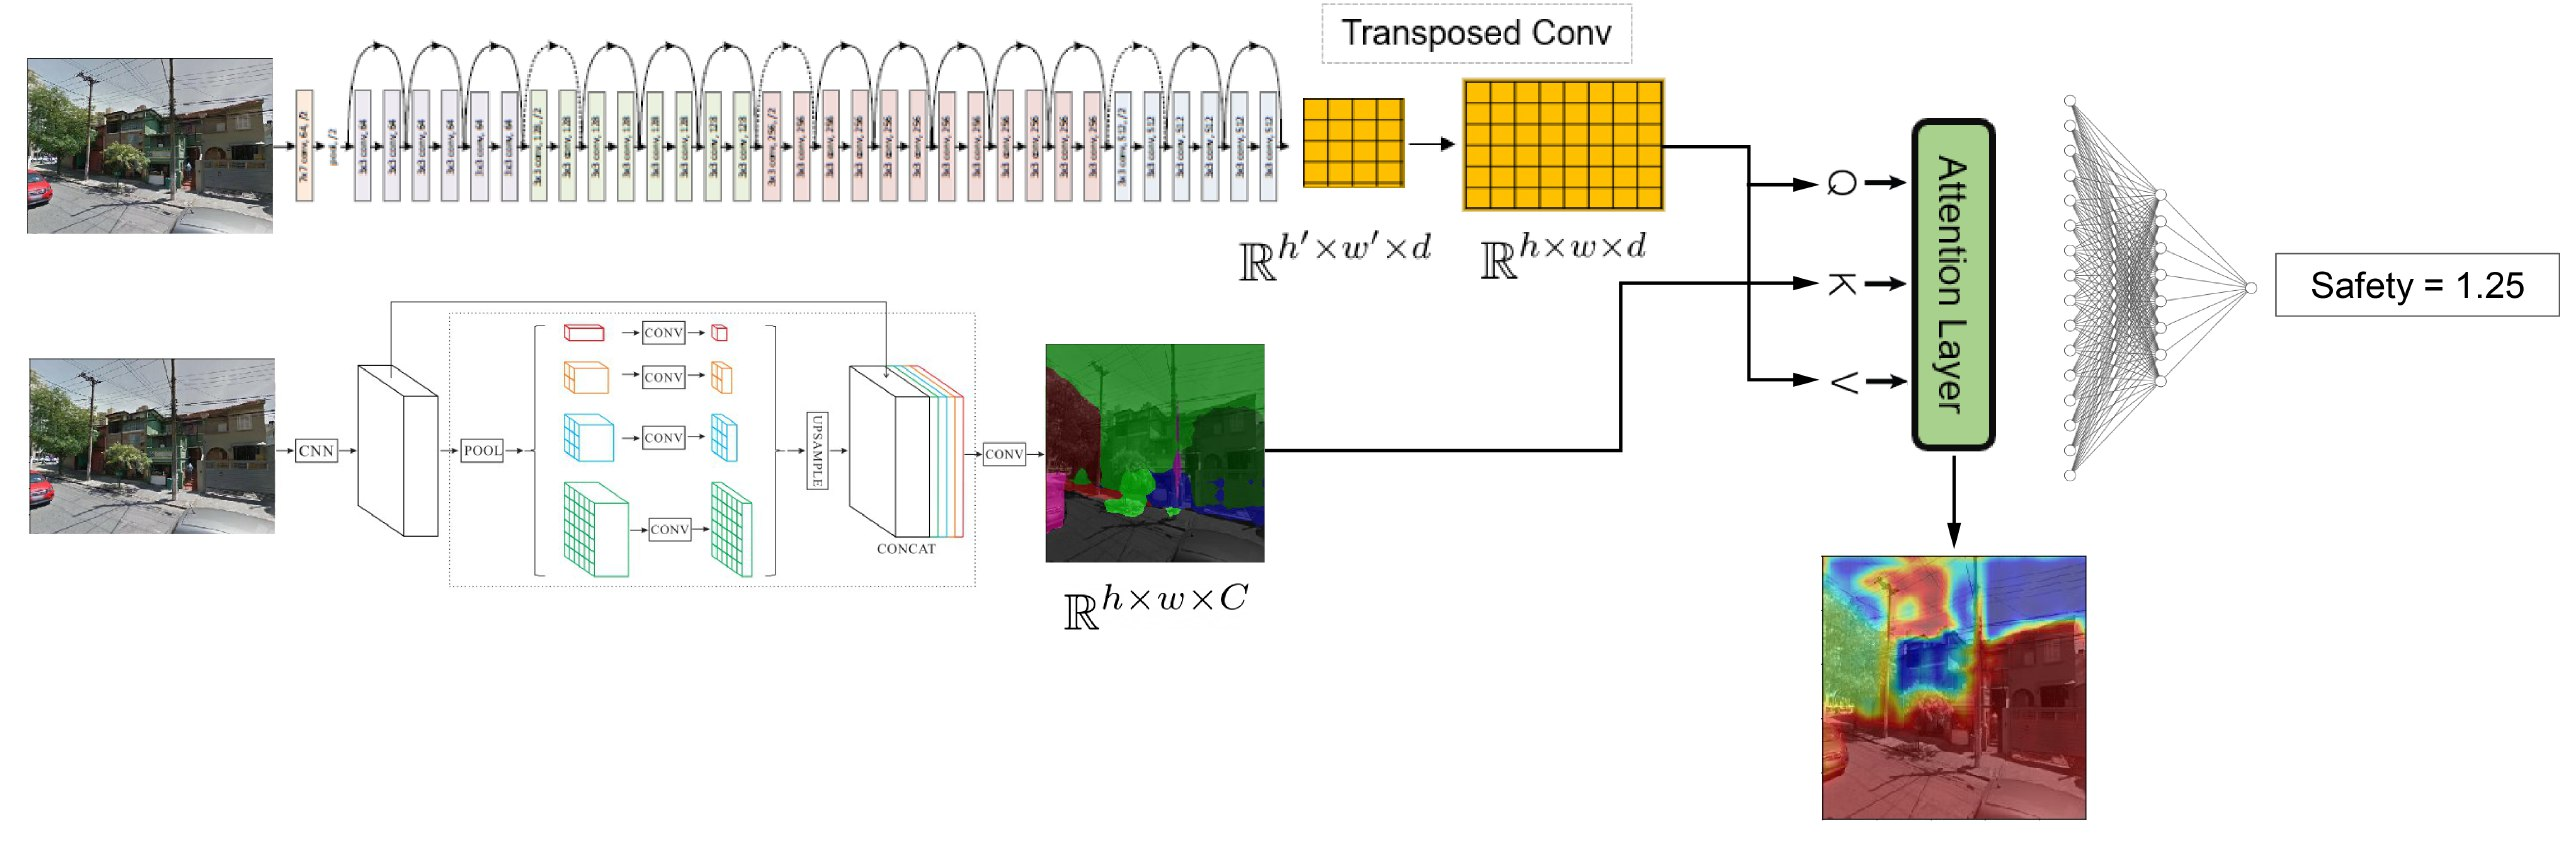
\includegraphics[width=1\textwidth]{./figures/segattn.png}
	\caption[Segmentation as key network]{Segmentation as key network.}
	\label{fig:segrank_1}
	\end{center}
\end{figure}

\section{Additional components}
\label{sec:adds}
\subsection{Loss function} \label{section:loss}
The loss function for this task must account for the pairwise structure of the dataset,
and should represent the cost of breaking restrictions given by equations
\ref{eq:constraints} and \ref{eq:constraints_ties}. For \ref{eq:constraints} we use
a hinge loss similar to the one proposed by \citeA{hidalgo_placepulse}:

\begin{equation}
	L_r(x_i,x_j,y | \Theta) = \max(0, -y(f_\Theta(x_i) - f_\Theta(x_j)) + m_r)
	\label{eq:r_loss}
\end{equation}

Where $f_\Theta$ and $\Theta$  represent the network and its parameters respectively, and $m_r$
is an hyperparameter. This loss component makes it so that the model learns to assign a higher
score to the image winner of the vote. Based on the work by \citeA{doughty_loss} we also add a second component so that tied votes can
be used for training. According with equation \ref{eq:constraints_ties} we define:

\begin{equation}
	L_t(x_i,x_j | \Theta) = \max(0, |f_\Theta(x_i) - f_\Theta(x_j)| - m_t)
	\label{eq:t_loss}
\end{equation}

Where $m_t$ is also an hyperparameter. Finally, the complete loss function is defined as:

\begin{equation}
	L(x_i,x_j,y | \Theta) =\left\{\begin{matrix}
		L_r(x_i,x_j,y)&\text{ if } y \in \{-1,1\} \\
		L_t(x_i,x_j)&\text{ if } y=0
	\end{matrix}\right.
\end{equation}

In practice we take the mean loss over the batch examples and we set $m_r=m_t=1$

\subsection{Semantic Dropout}
It's important to note that the semantic segmentation model trained on cityscapes,
presents an unavoidable drop in segmentation performance when applied on placepulse
due to domain shift. Errors in the segmentation can produce  significant problems
in the final perception quantification and can also cause confusing
attention heatmaps due to errors in the object edges.

In practice we identified a tendency for the models to have attention
weights highly biased towards specific segmentation classes, which is highly undesirable
both for explainability and model generalization.

We solve these problems by implementing what we call Semantic Dropout, similar to traditional Dropout \cite{srivastava_dropout},
but instead of dropping a single neuron with probability $p$, Semantic Dropout drops the
probabilities of an entire segmentation class, inducing artificial errors
during training and preventing the network from becoming too sensitive to
segmentation errors while also reducing the bias in attention weights. Mathematically
this technique is equivalent to the spatial dropout proposed in \citeA{tompson_efficient},
but applied to segmentation probabilities instead to convolutional kernels.

\begin{figure}[!htb]
	\minipage{0.25\textwidth}
		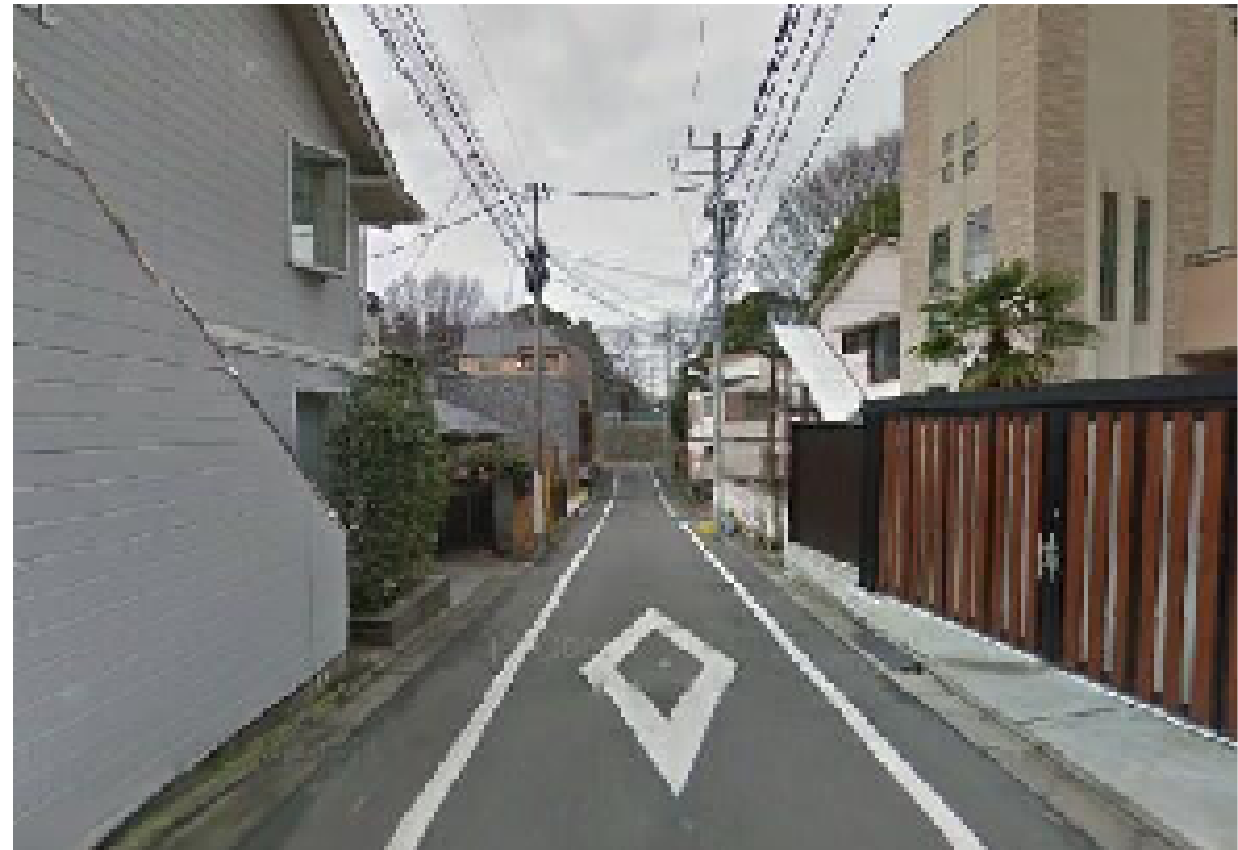
\includegraphics[width=\linewidth]{figures/original_sample.png}
	\endminipage\hfill
	\minipage{0.18\textwidth}
		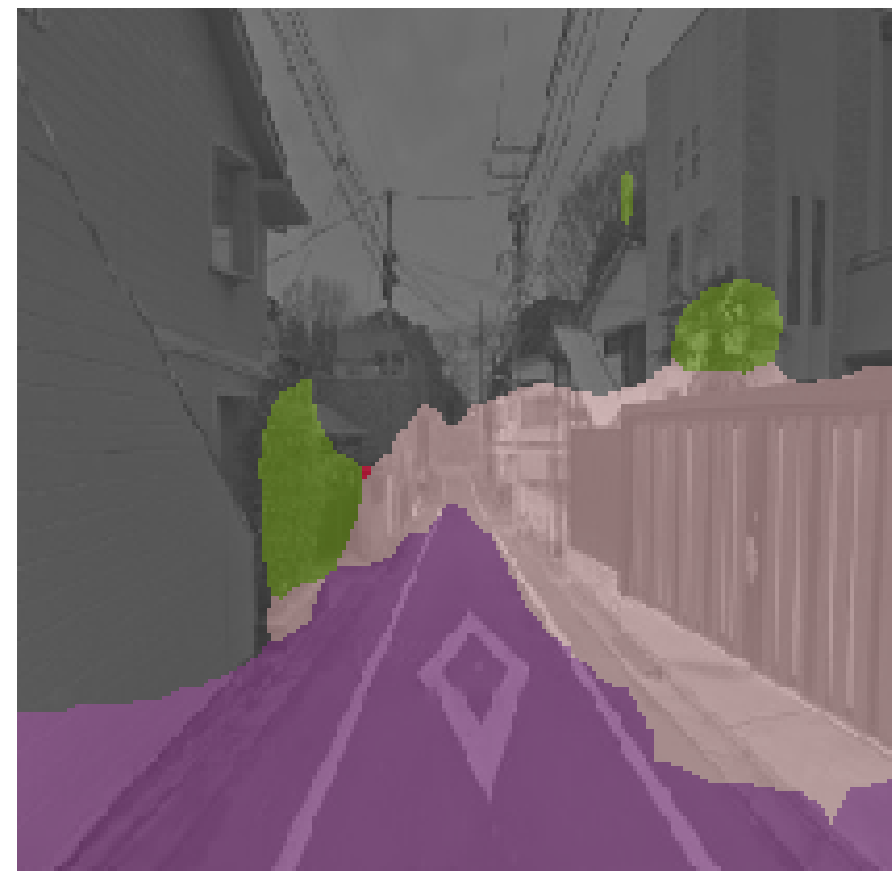
\includegraphics[height=\linewidth]{figures/segmentation_sample.png}
	\endminipage\hfill
	\minipage{0.26\textwidth}
		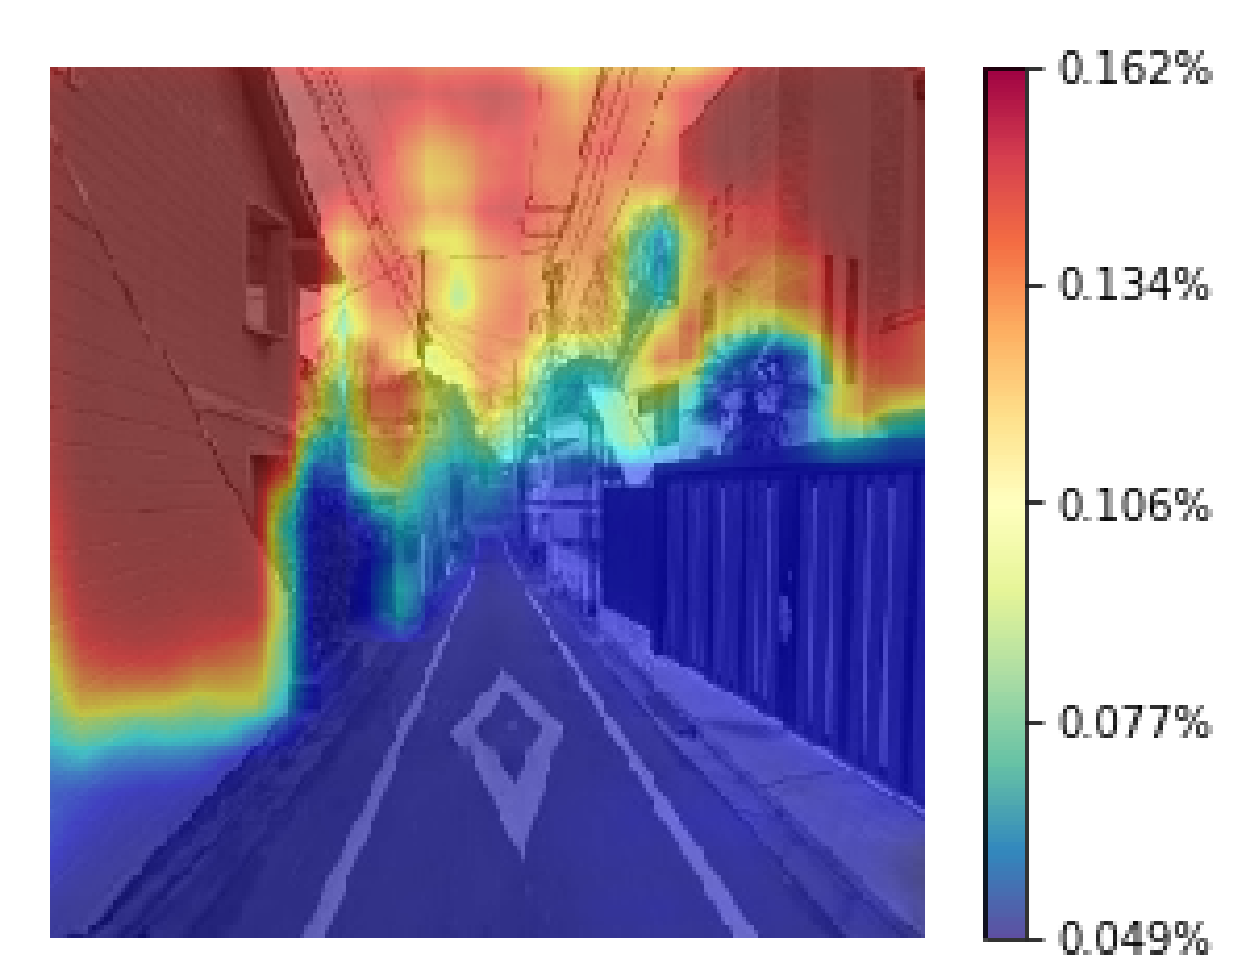
\includegraphics[width=\linewidth]{figures/segrank_sample.png}
	\endminipage\hfill
	\minipage{0.25\textwidth}
		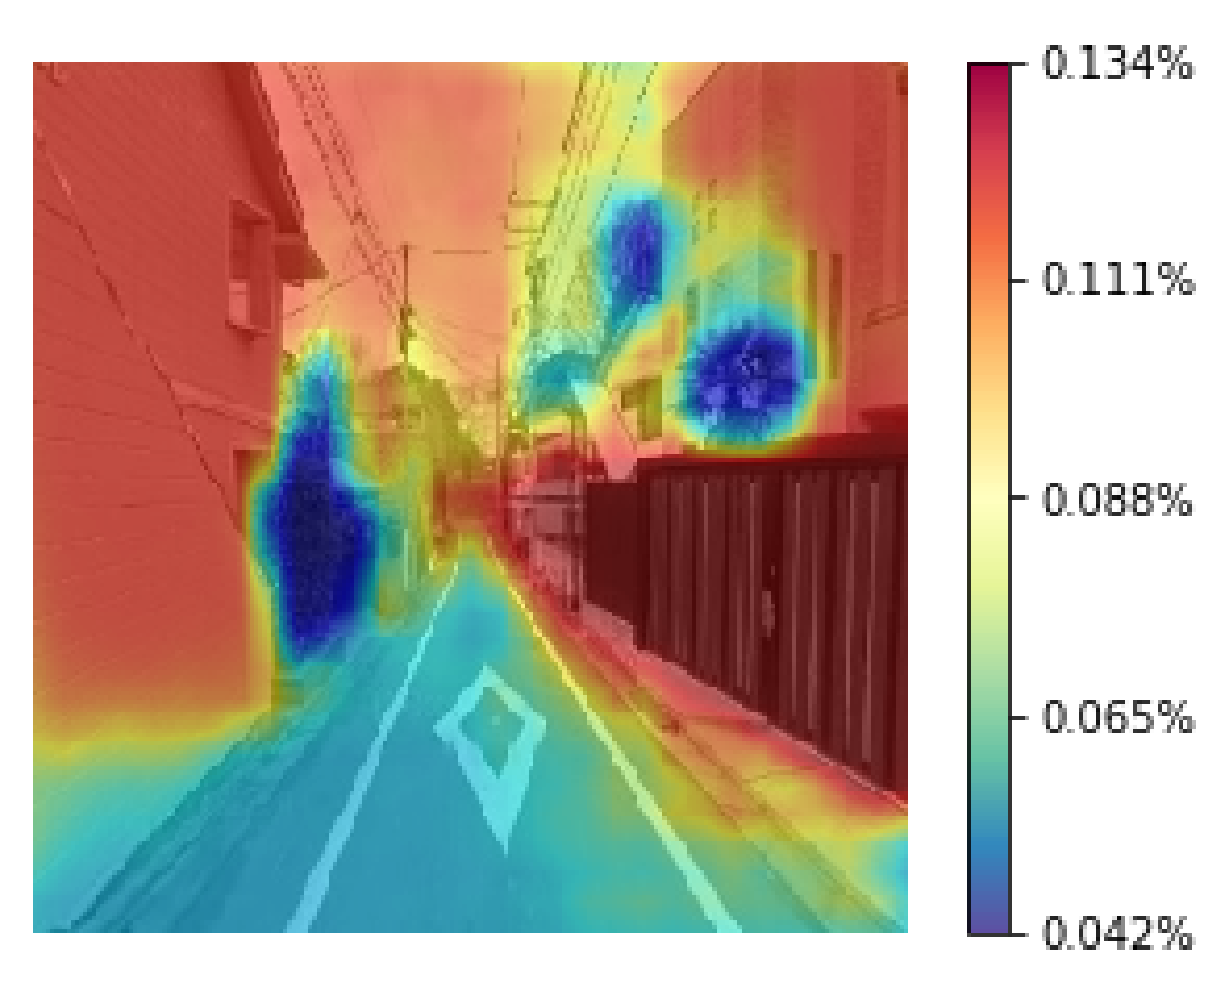
\includegraphics[width=\linewidth]{figures/segattn_sample.png}
	\endminipage
	\caption[Effect of Semantic Dropout]{
		Effect of Semantic Dropout. From left to right: original image, semantic segmentation
		and the outputs of the self attention model trained, without and with semantic dropout.
		The example shows how the attention weights are less biased towards one class and therefore
		less affected by the errors in segmentation.
	}
	\label{fig:dropout}
\end{figure}

\section{Baselines}
\label{sec:baselines}
With the purpose of making and ablation study, we also train two baseline models
based on the architecture proposed by \citeA{hidalgo_placepulse}, designed for
measuring the effect of the segmentation and attention mechanisms in both performance
and explainability of the models. We base these models on the ResNet50 CNN \cite{he_resnet},
as is the defacto approach for computer vision problems. We abstain from using larger
versions of ResNet due to significant overfitting issues.

\subsection{ResNet50 + MLP}
The first baseline consists of a standard finetuned ResNet50 with a two layer MLP. This
model doesn't provide any sort of out of the box explainability and therefore is useful
to measure how segmentation affects performance.
Unlike its segmentation based sibling, dropout and L2 regularization are necessary for training
this model, due to the significantly larger amount of trainable parameters that come from finetuning the CNN.

\subsection{ResNet50 + Self Attention layer + MLP}

A baseline on explainability is also important, since improving it is the key contribution
of this work. For that we use a similar architecture to attention-based explainability
models from the literature \cite{zhang_interpretable, cordonnier_relationship, bello_attention}, consisting on
combining a finetuned CNN with self attention layers.

We take the output of ResNet50's \textit{conv\_5c} layers and give it to the attention layer
defined in Section \ref{section:self-attn} and then to a two layer MLP for calculation of the final score.

\begin{figure}[ht]
	\begin{center}
	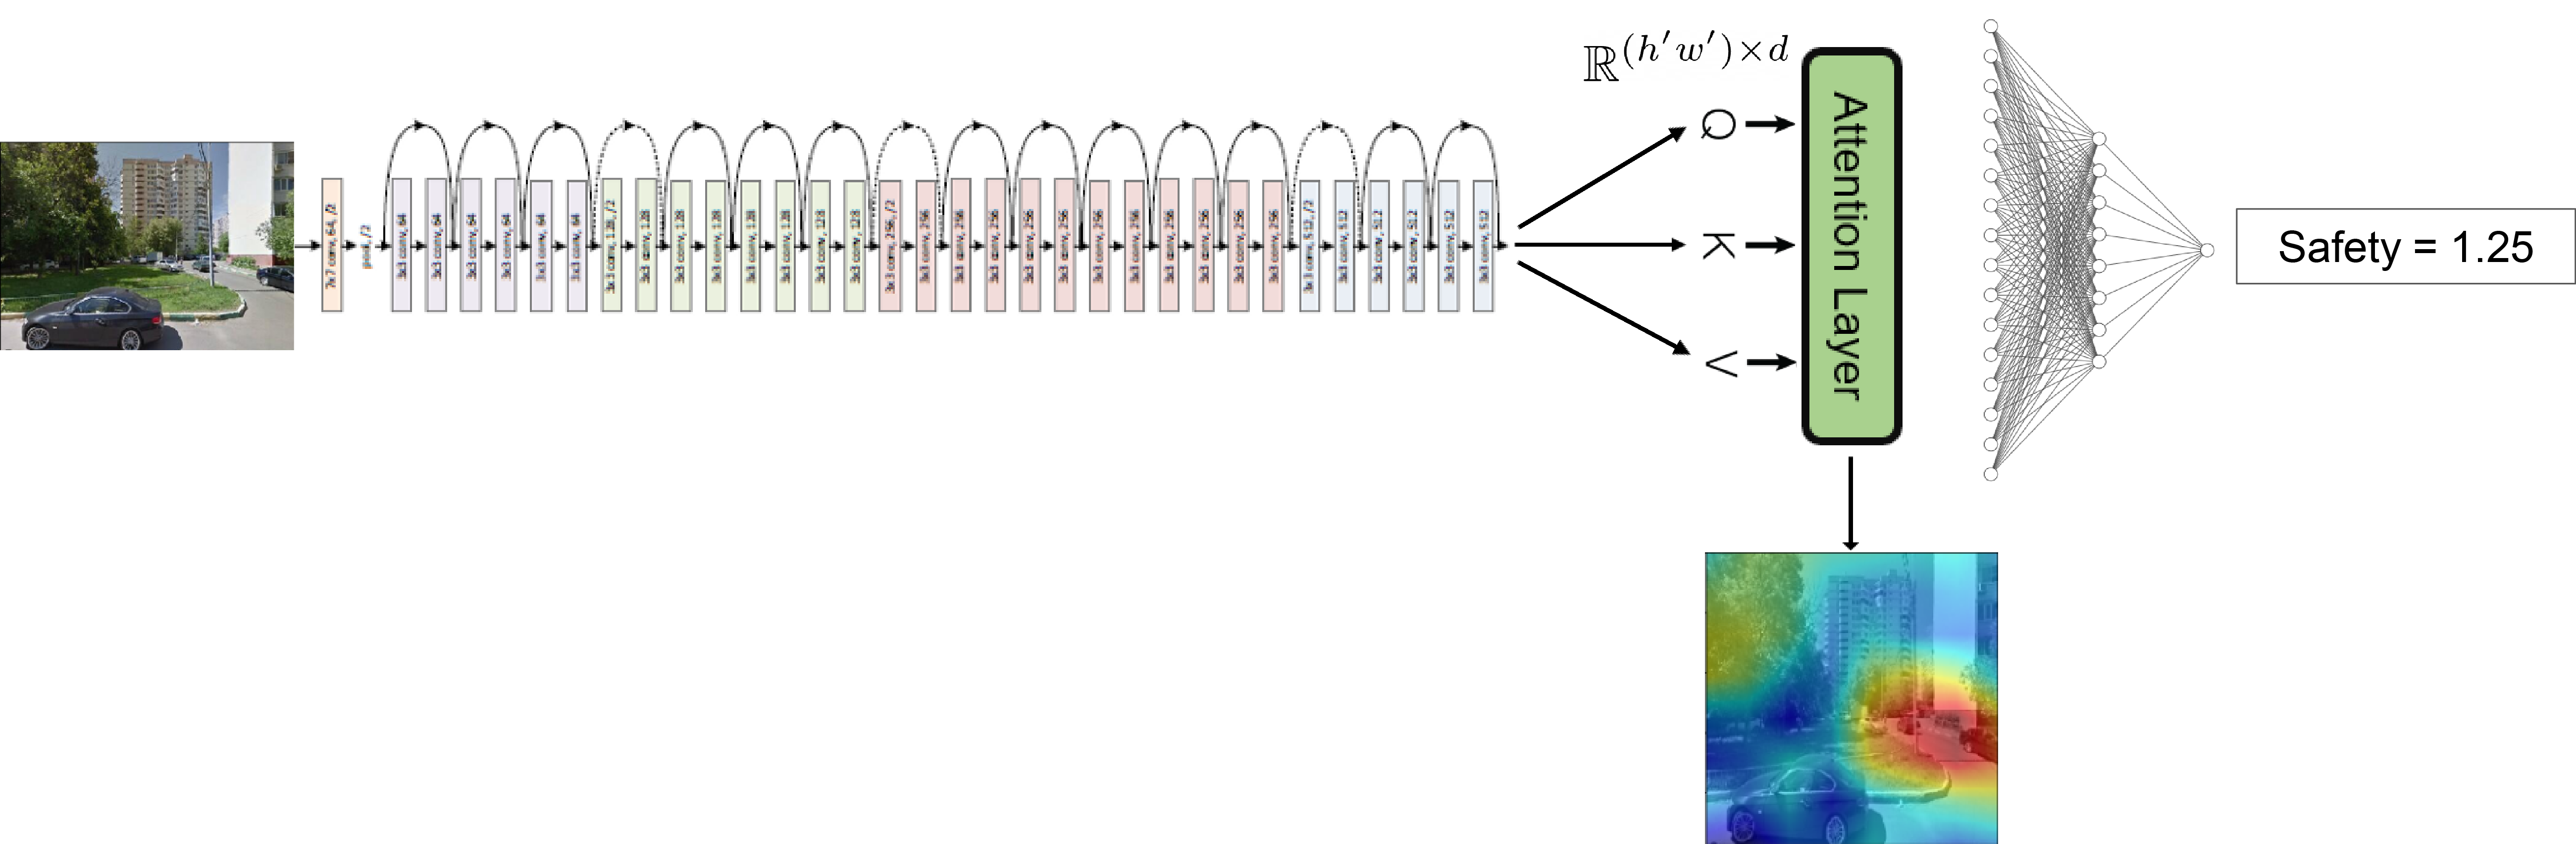
\includegraphics[width=1\textwidth]{./figures/attn_baseline.png}
	\caption[ResNet + SelfAttention]{ResNet and self attention network. ResNet diagram extracted from \citeA{he_resnet}.}
	\label{fig:attn_resnet}
	\end{center}
\end{figure}

\chapter[METHODOLOGY]{Methodology} \label{methodology}
This chapter shows the practical details of the implemented models and their
respective training process.

All of our models are implemented using the Pytorch library
\cite{paszke_pytorch} version 1.2.0.
We use the implementation and pretrained weights of ResNet
available on the Torchvision library \cite{marcel_torchvision}.
We train our own PSPNet based on the implementation by \citeA{huang_psp}.
All models are trained using a single 12 Gb Nvidia Geforce-GTX 1080 Ti GPU except
for the mixed model, which is trained on a 24 Gb Nvidia Titan RTX.

For training we make a 75\%/25\% train/validation splits of the dataset for
each attribute. We keep the splits fixed for all models, so they all see
and are evaluated on the same data. All models are trained for 40 epochs
and we keep the model with the best validation accuracy on epoch end.

\begin{table}[H]
    \begin{center}
        \caption[Hyper parameters]{Hyper parameters and configurations for each model.}
        \begin{tabular}{|l|r|r|r|r|r|}
            \hline
            \textbf{Parameter/Model} & \textbf{ResNet50} & \textbf{ResnetAttn} & \textbf{Seg}    & \textbf{Seg + Attn} & \textbf{Seg Att} \\ \hline
            Batch Size     & 32                           & 32                                & 32                         & 32                                   & 32                           \\
            Learning Rate  & $10^{-4}$                    & $10^{-4}$                         & $10^{-4}$                  & $10^{-4}$                            & $10^{-4}$   \\
            Opt. Algorithm & SGD                          & SGD                               & Adam                       & Adam                                 & Adam                         \\
            Finetuning     & Yes                          & Yes                               & No                         & No                                   & Yes                          \\
            Dropout        & 0.3                          & 0.3                               & 0                          & 0                                    & 0.1                          \\
            Semantic Dropout        & N/A                          & N/A                               & 0                          & 0.1                                    & 0.1                          \\
            Weight Decay   & $10^{-5}$                    & $10^{-5}$                         & 0                          & 0                            & 0    \\
            \hline
        \end{tabular}
        \label{tab:hyperparams}
    \end{center}
\end{table}

Baselines are trained with SGD with a momentum of $0.9$ \cite{rumelhart_backprop}
as it provided better results empirically. For segmentation based models we train with
Adam \cite{kingma_adam} and we set $\epsilon$, $\beta_1$ and $\beta_2$ to $10^{-9}$, $0.9$ and $0.98$ respectively.
We use semantic dropout on both models that have segmentation and attention, and add
an equivalent regular dropout layer to the ResNetAttn Baseline for fair comparison.
Weight decay and traditional dropout are used for all baseline models that finetune ResNet weights.
See table \ref{tab:hyperparams} for details on the training hyperparameters.


\chapter[RESULTS]{Results} \label{results}
This chapter shows the main results obtained. On section one we present the quantitative
performance and training results. Section 2 explains how the different visualizations
are generated, including examples for all the models.

\section{Quantitative results}

\subsection{Model performance}

Even though the objective of this research is to learn a ranking (or regression) to
quantify the urban perception, exact labels for this are not available, so we have to measure
model performance based on the Place Pulse votes, which as was mentioned on section
\ref{sec:problem_def}, has considerable issues. We use as performance measure the
equivalent to classification accuracy, considering which image won the vote as the target label.
In other words, we evaluate the percentage of restrictions (see \ref{eq:constraints})
that are satisfied by the model. We do this separately for each attribute in it's corresponding
validation set and the final accuracy value for each model is calculated as the mean accuracy through
all attributes.

Both ResNet based baseline models achieve an accuracy of \texttildelow 66\% and
as it was expected, replacing the more expressive CNN features for semantic segmentation,
caused a significant performance drop, falling to 60.62\% for SegRank and 61.43\% %TODO: update that value
for SelfSegRank. %TODO: AttnSegRank.
See table BLABLA, for the exact accuracy values.

\subsection{Training behavior}

Models trained on the place pulse dataset are very prone to overfitting, we believe this is due to it
having a very large amount of votes in comparison to the amount of available images, and because the task
is very hard to generalize given the high amount of noise that the dataset has from how it was collected.
This can be seen clearly on figures \ref{fig:resnet_graph} and \ref{fig:resnet_attn_graph}. Both
baselines models present considerably overfitting, showing accuracy differences between seen and unseen data
of up to 25\%, and ceasing to improve on the validation set after one or two training epochs.

\begin{figure}[ht]
	\begin{center}
	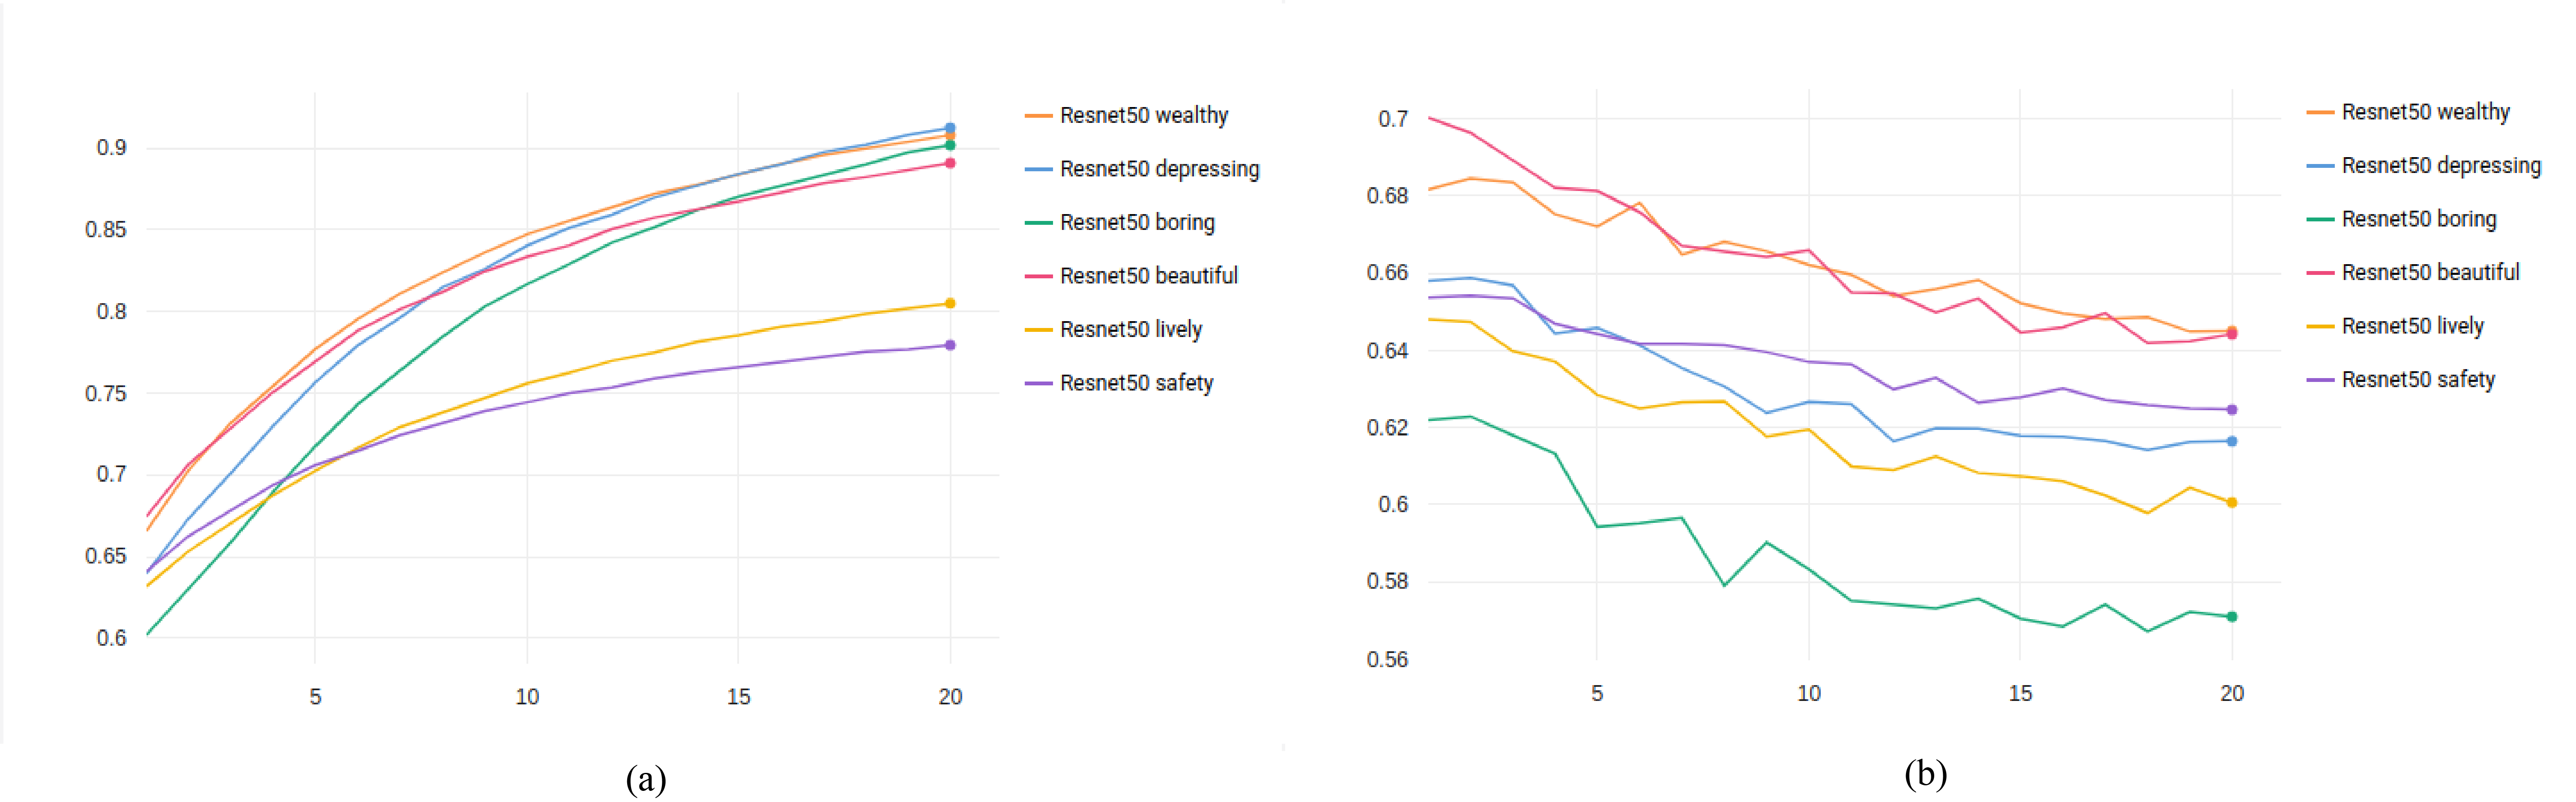
\includegraphics[width=1\textwidth]{./figures/resnet50_graph.png}
	\caption[ResNet Training curves]{
        ResNet50 baseline accuracy vs epoch learning curves on training (a) and validation (b).
        }
	\label{fig:resnet_graph}
	\end{center}
\end{figure}

\begin{figure}[ht]
	\begin{center}
	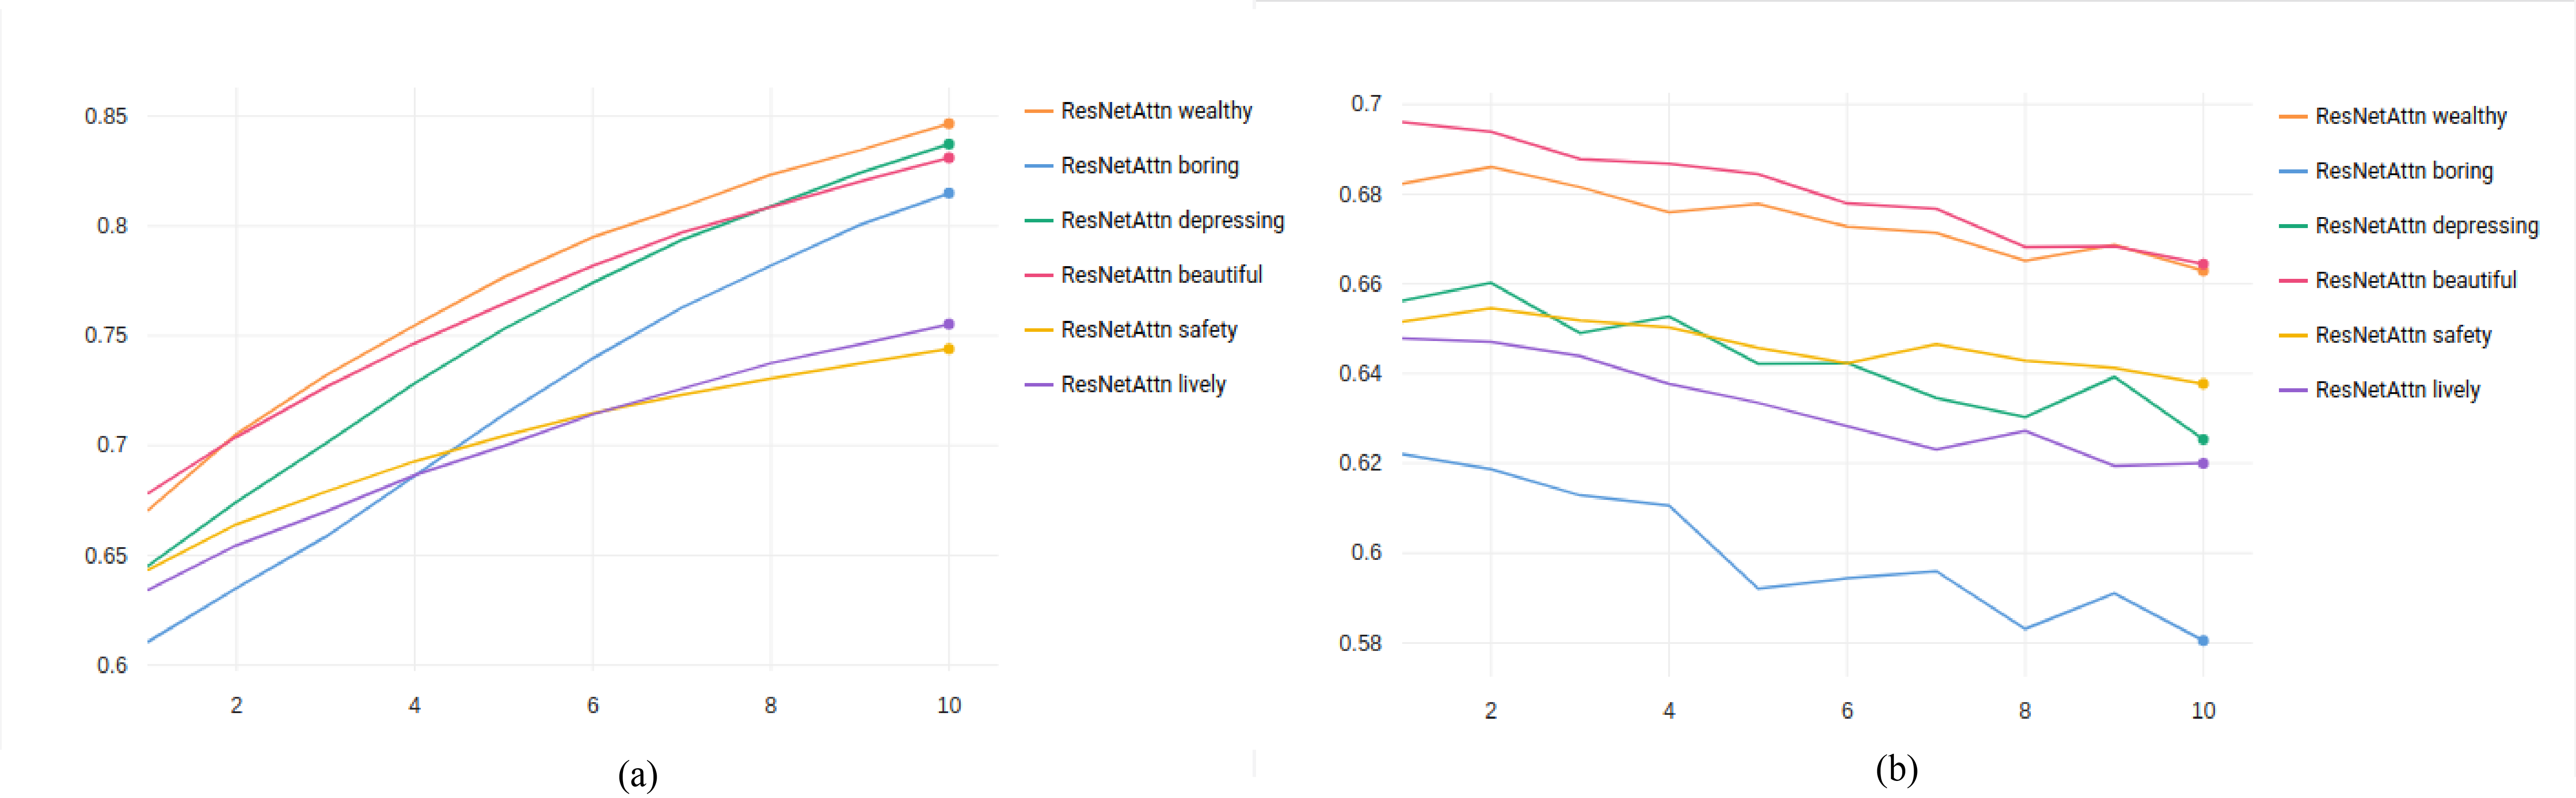
\includegraphics[width=1\textwidth]{./figures/resnet_attn_graph.png}
	\caption[ResNetAttn Training curves]{
        ResNetAttn baseline accuracy vs epoch learning curves on training (a) and validation (b).
        }
	\label{fig:resnet_attn_graph}
	\end{center}
\end{figure}

Replacing the CNN features for semantic segmentation generates a considerable change in training
behavior, with the reduced expressiveness of the segmentation acting as a very strong regularizer,
overfitting completely disappears, which translates to a drop of around 20\% to 30\% accuracy in training,
but of only 6\% on validation.

The basic SegRank architecture still reaches convergence after one or two epochs.
Adding the self attention layer makes it slightly slower allowing the model reach a higher validation accuracy.


\begin{figure}[ht]
	\begin{center}
	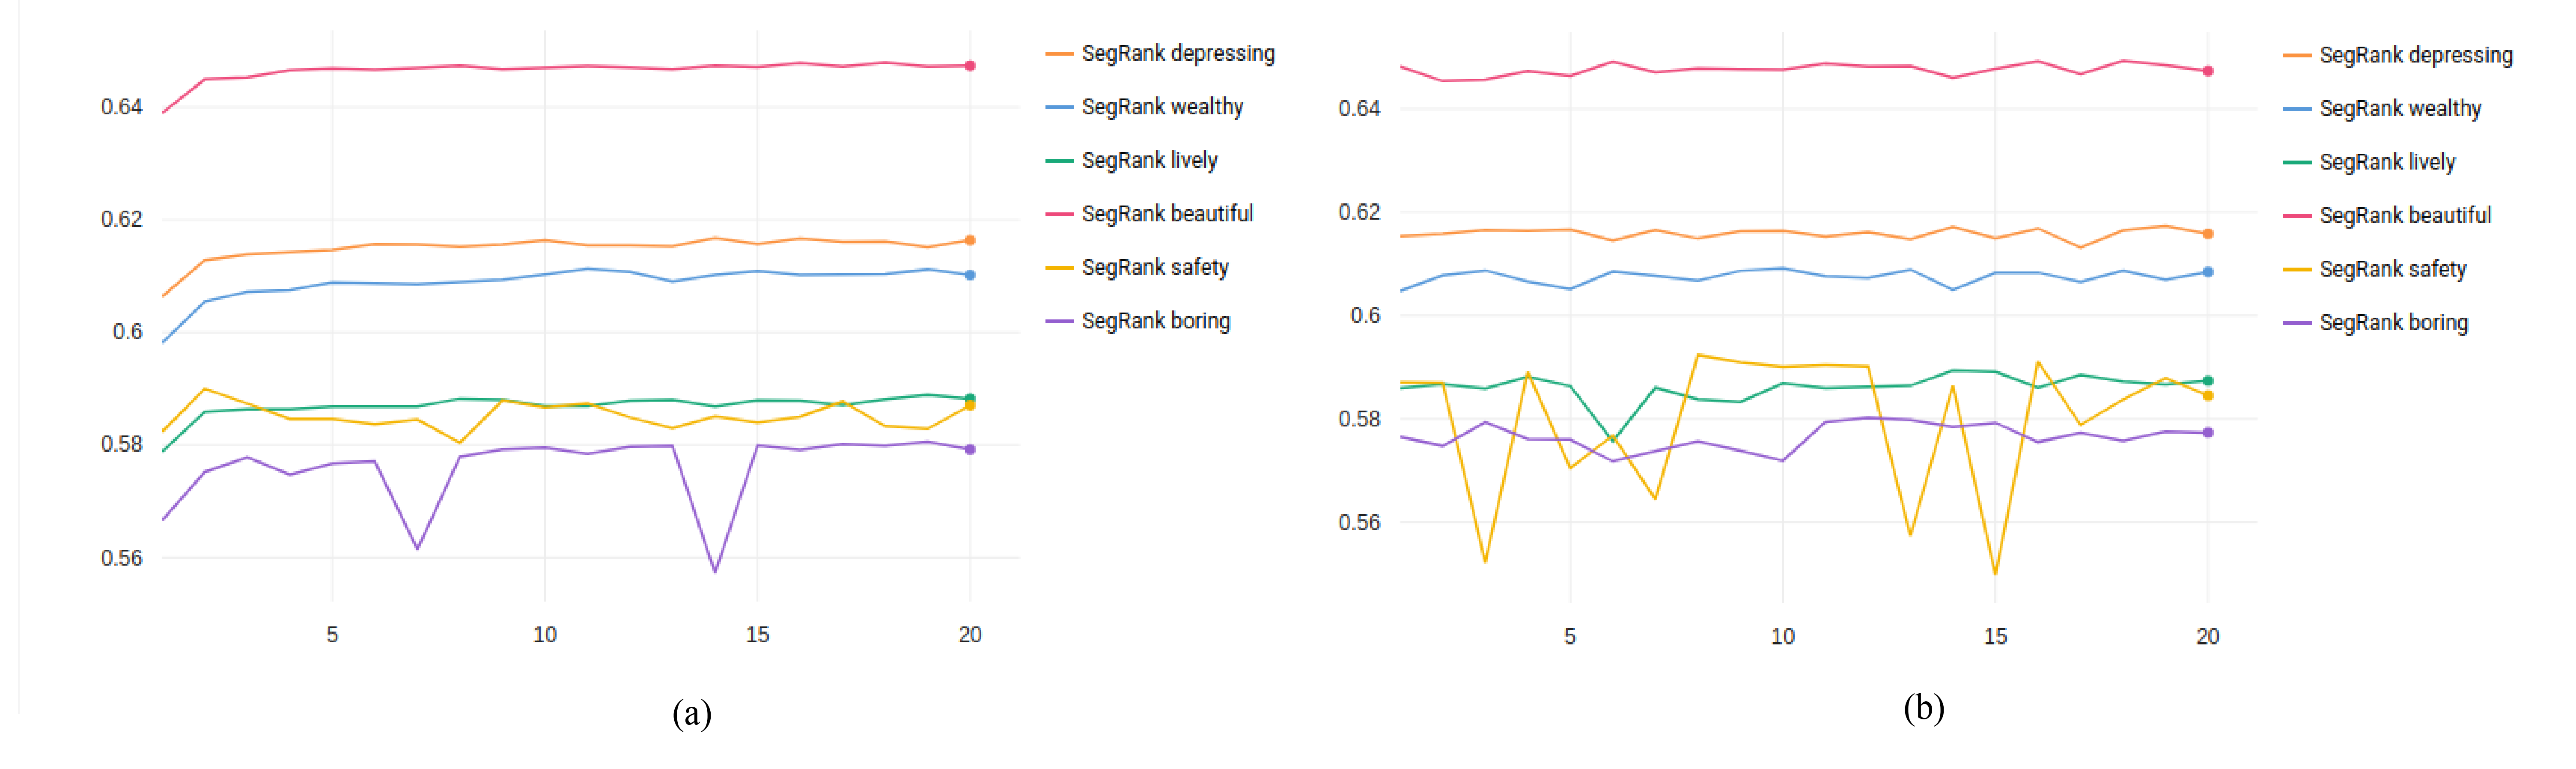
\includegraphics[width=1\textwidth]{./figures/segrank_graph.png}
	\caption[SegRank Training curves]{
        SegRank accuracy vs epoch learning curves on training (a) and validation (b).
        }
	\label{fig:segrank_graph}
	\end{center}
\end{figure}

\begin{figure}[ht]
	\begin{center}
	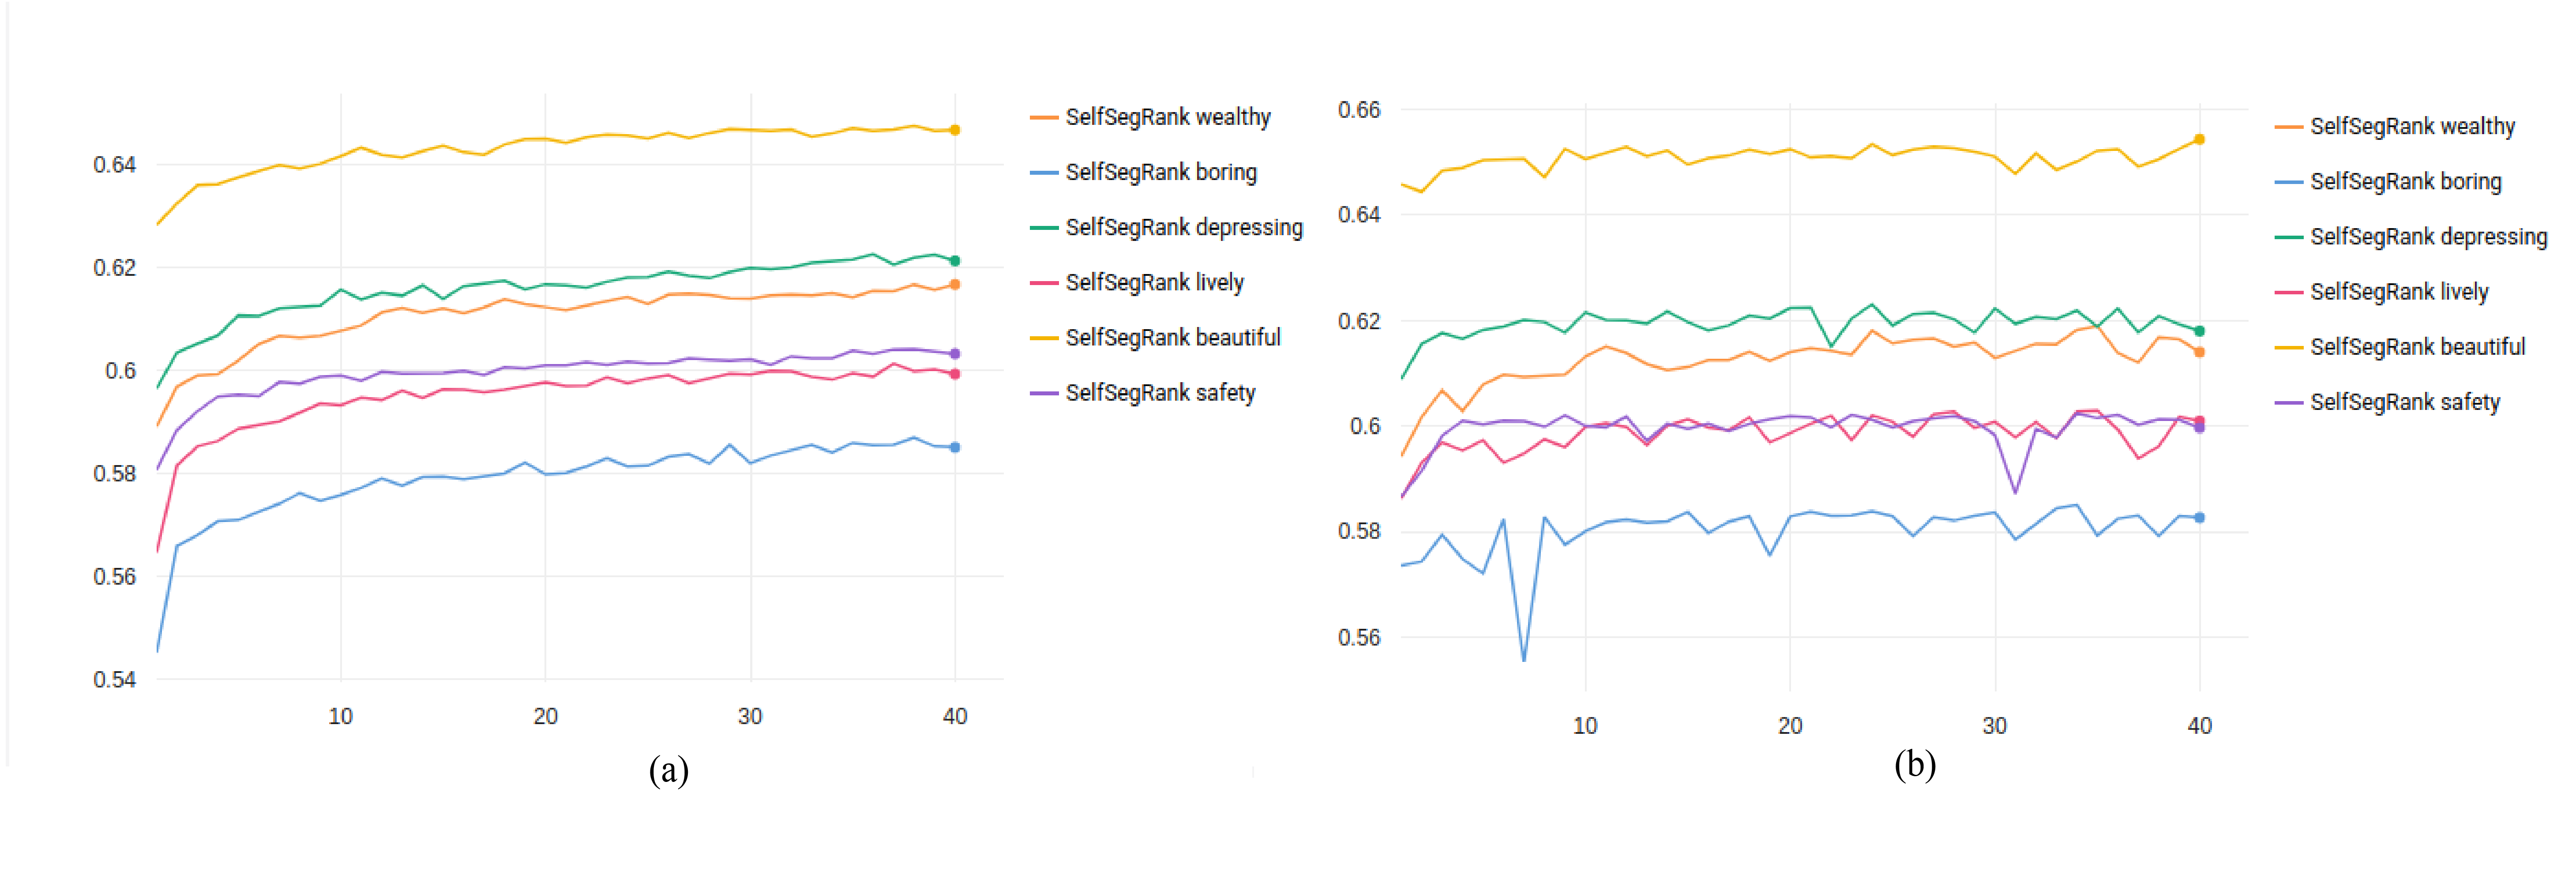
\includegraphics[width=1\textwidth]{./figures/selfsegrank_graph.png}
	\caption[SelfSegRank Training curves]{
        SelfSegRank accuracy vs epoch learning curves on training (a) and validation (b).
        }
	\label{fig:selfsegrank_graph}
	\end{center}
\end{figure}

As it can be seen on the results of all models, the learning process is consistent through out
the different attributes. The accuracy of the different attributes is also consistent across the
different models, with boring and beautiful being the hardest and easiest tasks to learn respectively
on all models.


\section{Visualization results}
\label{sec:visualization_results}

- Per attribute visualizations.

- Per object visualizations

- Baseline vs segrank vs segattn

\chapter[DISCUSSION]{Discussion} \label{discussion}
In this chapter we will do further analyses of the model results with particular
emphasis on the AttentionSegRank architecture due to it's better performance
and explainability. On section one we will discuss the effects of using semantic segmentation
on neural network  training. Section 2 will show the quantitative relationship between
segmentation, attention and the perception quantification. And finally, section 3 we will
analyze the implications of this method on model explainability.

\section{Effect of semantic segmentation on learning}
As was already mentioned on section \ref{sec:training}, adding a fixed segmentator to
the neural network architecture resulted in a reduction of performance along with a considerable
reduction of overfitting. The behavior was expected when fully replacing the CNN features,
due to the reduced expressiveness of the segmentation and the lack of finetuning, but
unexpectedly, although it is reduced, this behavior persists when combining the fixed
segmentation with the finetuned ResNet50 through the attention layer. We conclude from this
that restricting the attention weights to the shapes and classes given by the segmentation
has a regularizing effect on learning, reducing the model capacity even when the amount of trainable
weights is maintained.

In the case of the PlacePulse dataset this is not a problem since
all traditional deep models suffer of significant overfitting. It remains an interesting research
question  if these behavior will transfer to other tasks and datasets.



\section{Relationship between urban perception and semantic segmentation}

\section{Relationship between urban perception and attention}

\section{Effect of attention over semantic segmentation on model explainability}

\chapter[CASE STUDY]{Case study} \label{case_study}
In order to do a practical evaluation of the model's performance and an assessment
of the model's applicability, most of the recent literature include a case study
for  a particular city \cite{rossetti, zhang_measuring, zhang_uncovering, quercia_aesthetic,tamara_judgments,liu_machine}.
We continue this trend and use the AttnSegRank models trained on placepulse
to analyze ~120,000 Google Street View images of Santiago de Chile.

We use the results to generate a visualization of the city showing how the perception
attributes behave through out the different sectors. These are shown in figure
\ref{fig:colormaps}, and is easy to see how they precisely replicate the city's actual
income distribution, shown on figure \ref{fig:eod}. Santiago is known for a considerably
segregated urban distribution, in which the wealthier classes, and a large portion
of goods and services are concentrated in a cone extending from the center of the city
to the north east \cite{sabatini_segregacion}, due to that the 6 attributes show a
highly similar pattern that reflect that reality very well.

Some interesting insights are that as it was mentioned on section \ref{sec:seg_explainability},
highways and long roads are marked as very boring, which can be seen on the intense
red lines present on the boring attribute, and that the more lively places (and the less boring)
are much more concentrated towards the center of the city than the north east corner, which
we believe is due to this sectors being the most busy in the city, with constant flow
of cars and people at all times while also having a good amount of green areas.

\begin{figure}[ht]
	\begin{center}
	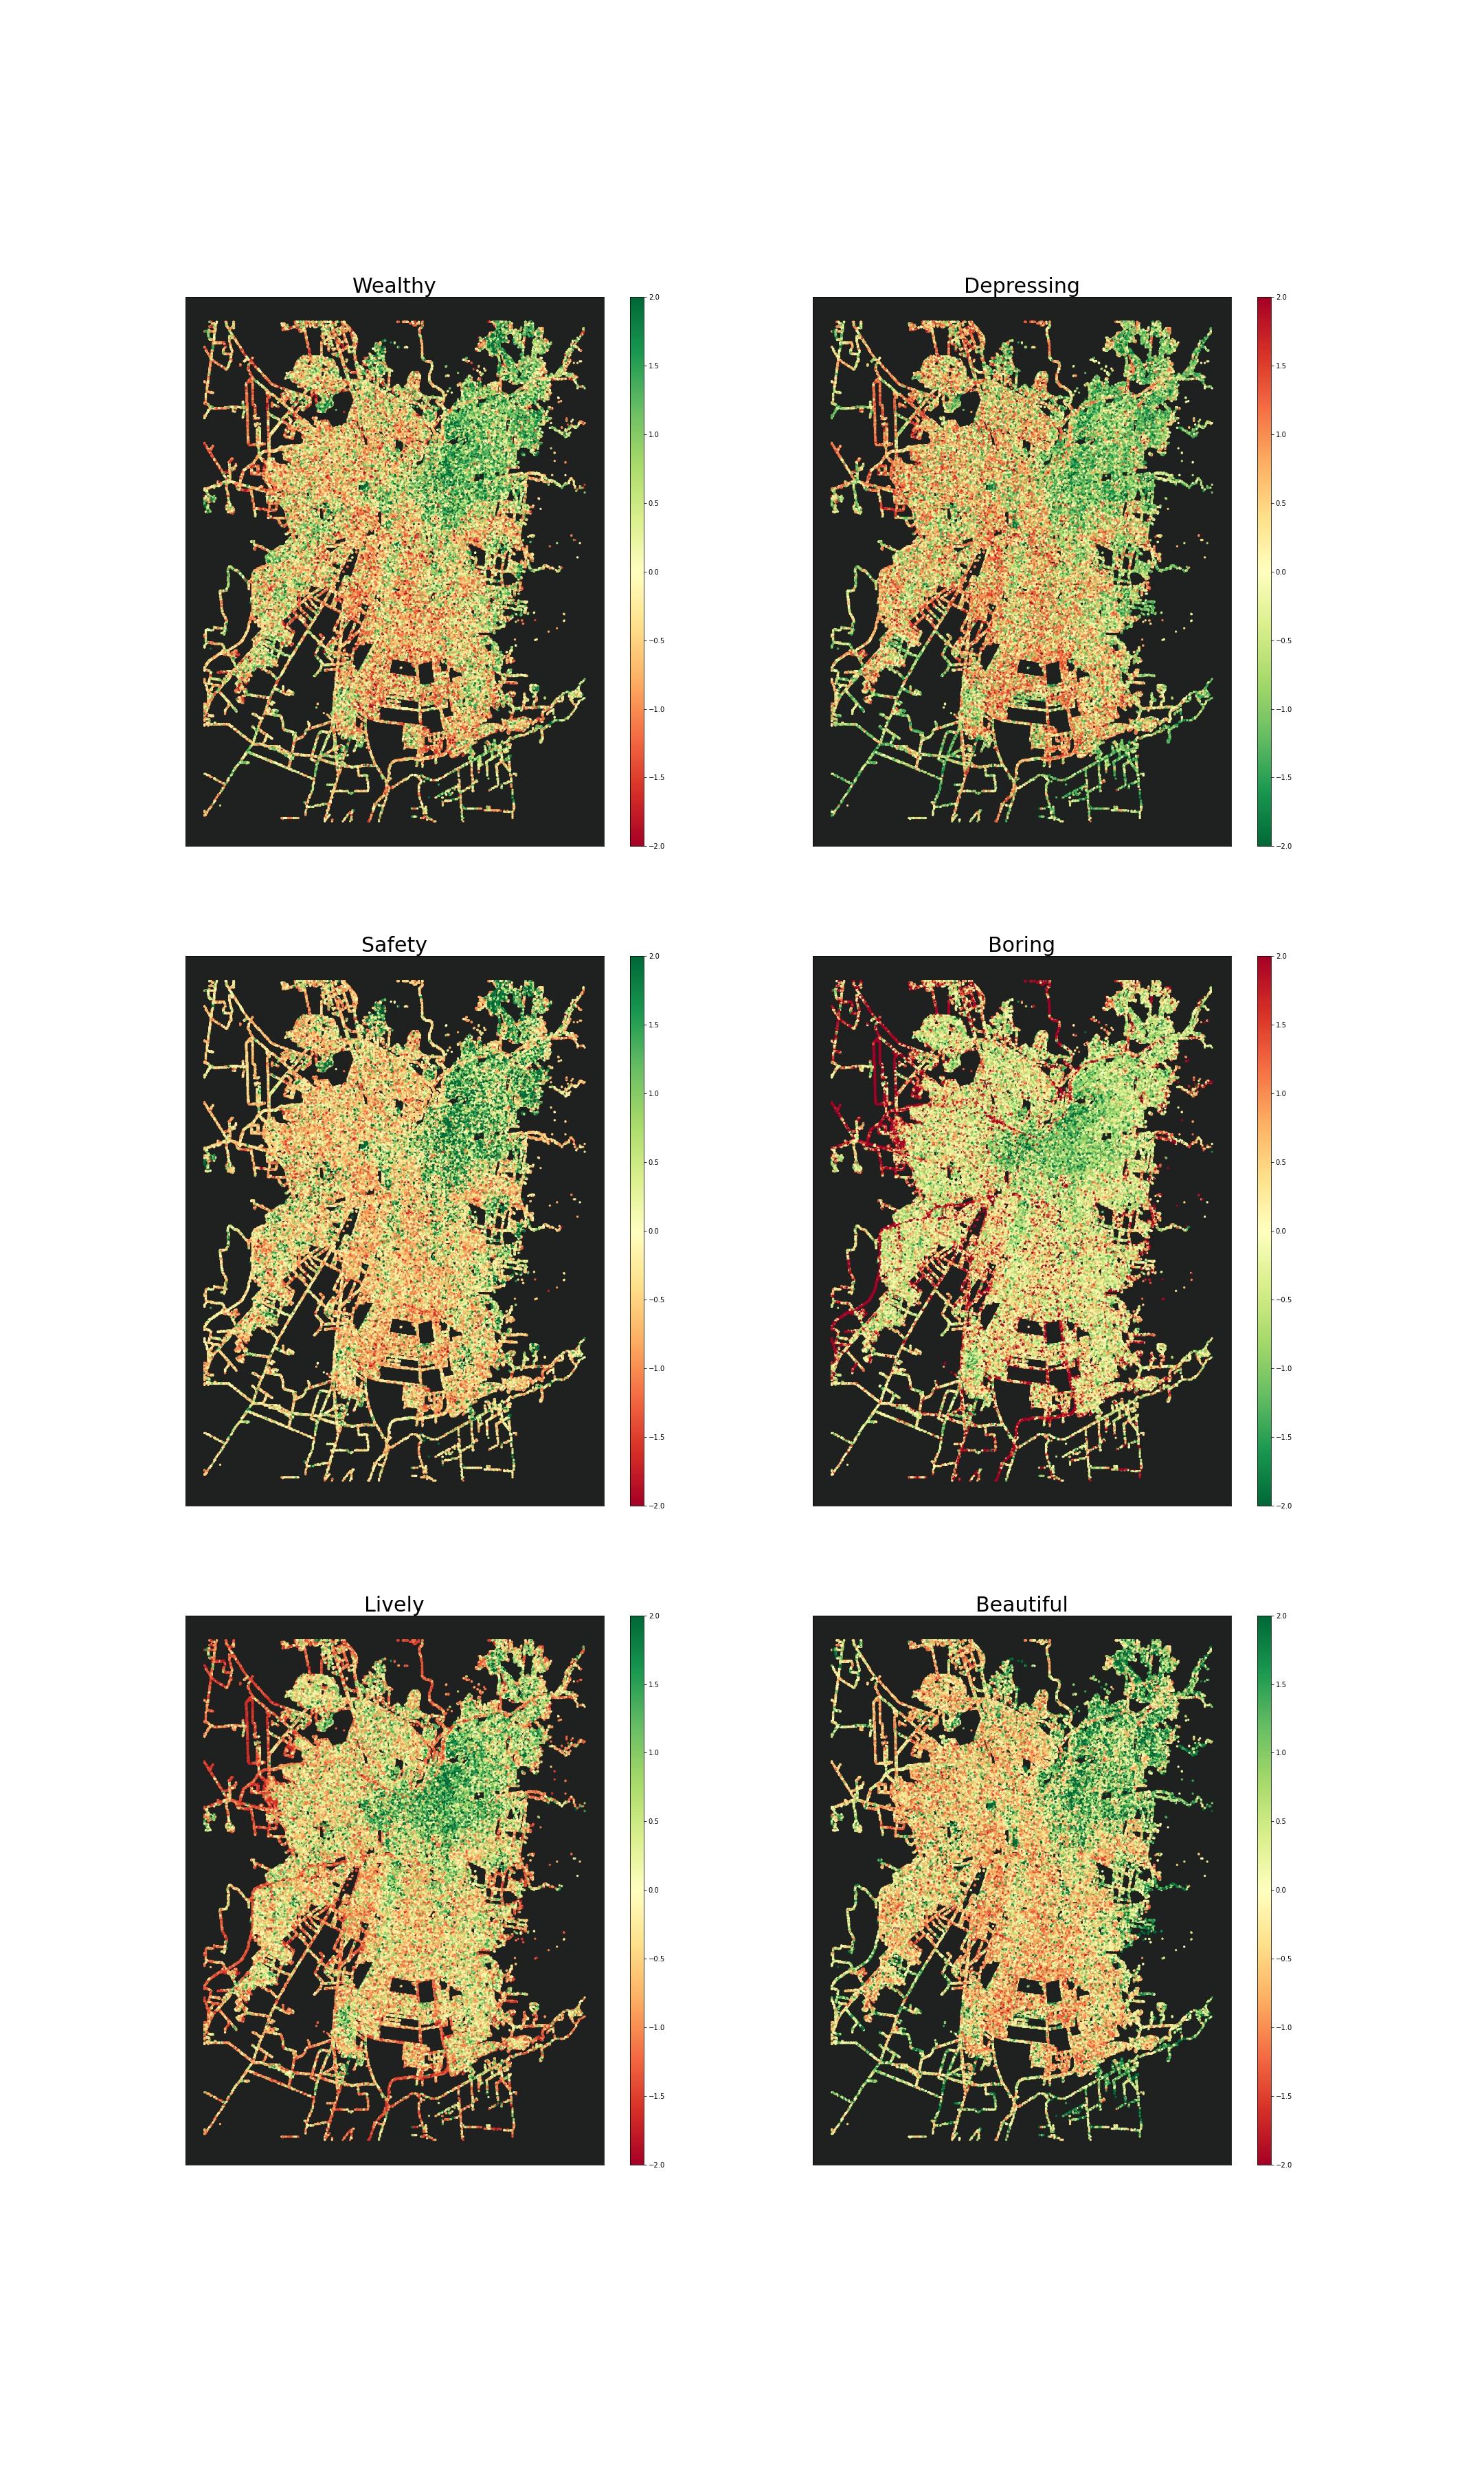
\includegraphics[width=0.75\textwidth]{./figures/colormaps.jpg}
	\caption[Urban Perception for Santiago de Chile]{
        Urban Perception for Santiago de Chile, each dot represents an image that
        was analyzed with our model.
    }
	\label{fig:colormaps}
	\end{center}
\end{figure}


\begin{figure}[ht]
	\begin{center}
	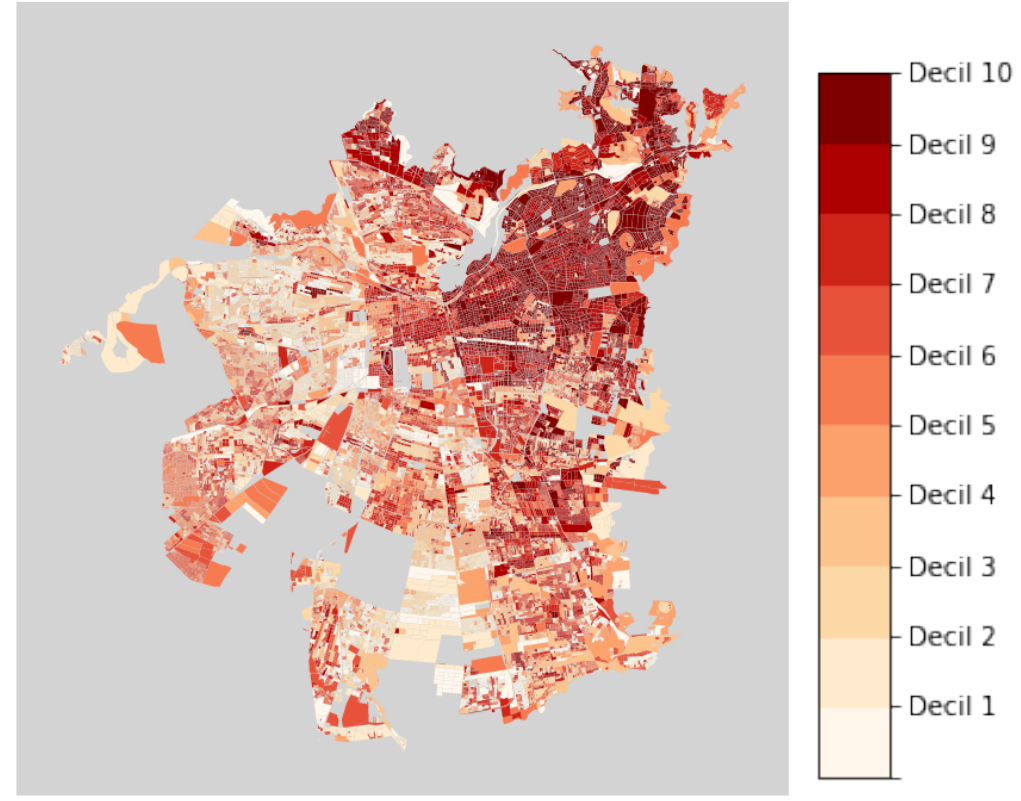
\includegraphics[width=0.75\textwidth]{./figures/eod.png}
	\caption[Wealth distribution of Santiago de Chile]{
        Wealth distribution of Santiago de Chile by deciles. Darker means wealthier.
        Reproduced from \citeA{Ramirez2020}.
    }
	\label{fig:eod}
	\end{center}
\end{figure}

In order to have a quantitative measure of the ranking generated for Santiago we calculate the mean score over
the images of each commune in the city and compare the results with their respective
socioeconomic indicators. We find a strong correlation between our perceived wealthy score
and the poverty rate, and between our perceived depressiveness score and social vulnerability.
We show this results on figures \ref{fig:poverty} and \ref{fig:vulnerability}.

\begin{figure}[ht]
	\begin{center}
	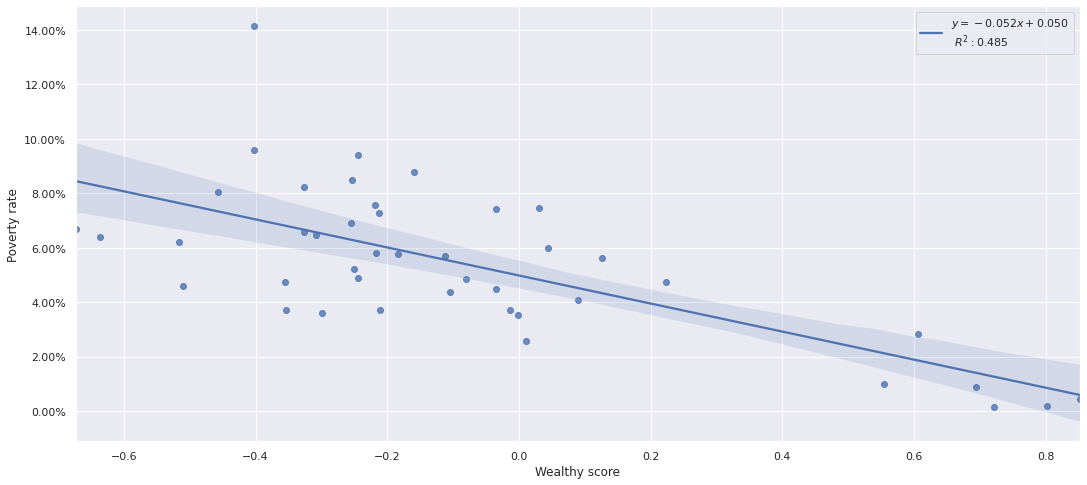
\includegraphics[width=0.75\textwidth]{./figures/poverty_rate.png}
	\caption[Poverty rate vs perceived wealthy score]{
		Poverty rate vs perceived wealthy score by commune in Santiago de Chile.
		Data taken from \citeA{casen}.
    }
	\label{fig:poverty}
	\end{center}
\end{figure}

\begin{figure}[ht]
	\begin{center}
	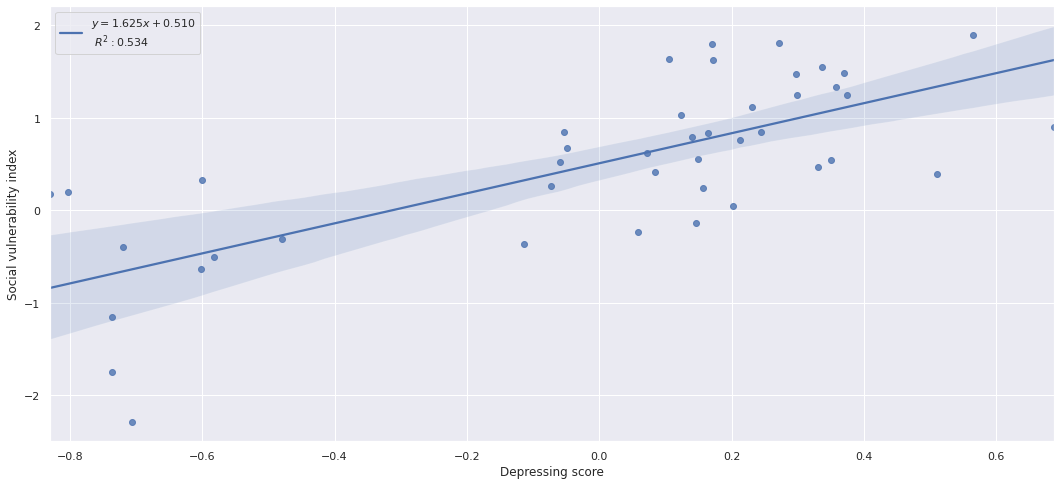
\includegraphics[width=0.75\textwidth]{./figures/vulnerability_index.png}
	\caption[Vulnerability index vs perceived depressiveness score]{
		Vulnerability index vs perceived depressiveness score by commune in Santiago de Chile.
		Data taken from \citeA{amuch}.
    }
	\label{fig:vulnerability}
	\end{center}
\end{figure}

\chapter[CONCLUSIONS]{Conclusions} \label{conclusions}
Nothing to say. Be happy.

\section{Contribution to the state of the art}

%%%%%%%%%%%%%
%       REFERENCES        %
%%%%%%%%%%%%%

\cleardoublepage
\phantomsection \label{references}
\bibliographystyle{apacite}
\renewcommand{\bibname}{REFERENCES}

%%%% ACTIVAR SIGUIENTES 3 LINEAS SI POSTGRADO RECHAZA LA BIBLIOGRAFIA
%\setlength{\bibleftmargin}{0em}
%\setlength{\bibindent}{0em}
%\setlength{\bibitemsep}{1em}


\bibliography{Thesis}

%%%%%%%%%%%%
%      APPENDICES      %
%%%%%%%%%%%%

\appendix % It is like a chapter, so each appendix (A, B, C...) must to be considered as a section

\newpage
\section[Semantic Segmentation]{Semantic Segmentation}
\subsection{Visual representation}
\label{sec:seg_colors}
For visually representing segmentation, we make a color map over the images, following
the cityscapes color palette \cite{cordts_cityscapes}. See figure \ref{fig:segmentation_colors}
for the exact palette and class list, and figure \ref{fig:cs_sample} for an example.

\begin{figure}[ht]
	\begin{center}
	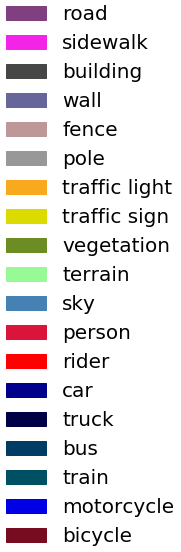
\includegraphics[width=0.2\textwidth]{./figures/seg_colors.png}
	\caption[Segmentation color palette]{
        Segmentation color palette.
        }
	\label{fig:segmentation_colors}
	\end{center}
\end{figure}

\begin{figure}[ht]
	\begin{center}
	\includegraphics[width=1\textwidth]{./figures/cityscapes_sample.png}
	\caption[CityScapes sample]{
        CityScapes sample.
        }
	\label{fig:cs_sample}
	\end{center}
\end{figure}

\subsection{Segmentation distribution}
\label{sec:seg_distribution}
Given the domain shift from Cityscapes to PlacePulse, is important to check how
the segmentation behaves on the new dataset.

The most significant difference between the datasets is the image size, which are almost 13
times bigger in cityscapes, allowing for smaller objects like traffic signs to be clearly
distinguishable. In training CS images are used with size of $769 \times 769$, while
place pulse images are used with the standard $224\times224$. Another important difference
is the origin of the images, while Cityscapes images were all taken on different cities of
the same developed country (Germany), PlacePulse images come from 56 cities distributed on all
continents, including both developed and developing countries, with the later ones contributing
images with a significant visual difference.

Table \ref{tab:segmentation} show the percentage of pixels belonging to each segmentation class
on the entire set of images of the PlacePulse dataset. Evidently this are not ground truth labels,
but the ones obtained by our  PspNet trained on Cityscapes. As was expected, classes representing
physically smaller objects have an almost negligible contribution since the smaller image size renders
them pretty much unidentifiable. Domain shift makes the model constantly confuse the sidewalk (which can
be seen in a large percentage of PlacePulse images) with the main road, reducing the class presence
to a very underwhelming 0.96\%. Same behavior can be perceived with the terrain class.


\begin{table}[H]
	\begin{tabular}{|l|r|} \hline
	Segmentation Class & \% of pixels \\ \hline
	Building      & 26.60\% \\
	Vegetation    & 25.52\% \\
	Road          & 24.21\% \\
	Sky           & 6.24\%  \\
	Fence         & 5.09\%  \\
	Truck         & 2.96\%  \\
	Car           & 1.94\%  \\
	Person        & 1.48\%  \\
	Bicycle       & 1.36\%  \\
	Motorcycle    & 1.28\%  \\
	Sidewalk      & 0.96\%  \\
	Wall          & 0.89\%  \\
	Terrain       & 0.65\%  \\
	Pole          & 0.33\%  \\
	Train         & 0.26\%  \\
	Bus           & 0.14\%  \\
	Traffic sign  & 0.05\%  \\
	Traffic light & 0.02\%  \\
	Rider         & 0.02\%  \\ \hline
	\end{tabular}
	\caption[Segmentation Distribution]{
		Pixel distribution of the segmentation classes over the PlacePulse Dataset
	}
	\label{tab:segmentation}
\end{table}
\section[Significance Tables]{Significance Tables}\label{sec:sig_tables}
Here we present the full significance tables from the results discussed in section \ref{sec:significance}

\begin{table}[H]
	\begin{tabular}{|l|rrrrrrr|}
		\hline
					& \multicolumn{7}{c|}{\textbf{Significance \%}}   \\ \hline
		\textbf{Class}         & \textbf{Wealthy}        & \textbf{Depressing}     & \textbf{Safety}         & \textbf{Boring}         & \textbf{Lively}         & \textbf{Beautiful}      & \textbf{Average}        \\
		\hline
		Road          & 62.46          & \textbf{77.98} & \textbf{78.64} & 31.77          & \textbf{90.58} & 17.33        & \textbf{59.79} \\
		Building      & \textbf{63.74} & 9.21           & 30.35          & \textbf{82.69} & 17.99          & \textbf{52.79} & 42.80          \\
		Sky           & 43.81          & 44.51          & 39.34          & 18.34          & 45.68          & 45.80          & 39.58          \\
		Person        & 4.86           & 18.18          & 10.83          & 28.83          & 25.76          & 6.77           & 15.87          \\
		Car           & 4.09           & 19.70          & 12.02          & 34.63          & 6.12           & 15.50          & 15.34          \\
		Vegetation    & 4.27           & 22.56          & 20.57          & 5.50           & 5.45           & 24.08          & 13.74          \\
		Bicycle       & 4.81           & 8.25           & 10.32          & 15.48          & 16.57          & 10.10          & 10.92          \\
		Sidewalk      & 10.65          & 12.46          & 2.21           & 7.65           & 7.35           & 9.66           & 8.33           \\
		Truck         & 4.65           & 11.38          & 2.94           & 9.57           & 6.29           & 14.29          & 8.19           \\
		Motorcycle    & 4.92           & 5.31           & 6.68           & 8.10           & 9.77           & 10.97          & 7.63           \\
		Wall          & 3.43           & 4.63           & 4.90           & 9.95           & 5.33           & 9.14           & 6.23           \\
		Fence         & 5.33           & 13.15          & 6.83           & 1.75           & 2.17           & 4.55           & 5.63           \\
		Pole          & 1.48           & 2.76           & 2.04           & 8.00           & 13.03          & 3.49           & 5.13           \\
		Terrain       & 0.74           & 2.72           & 2.72           & 13.31          & 1.45           & 4.38           & 4.22           \\
		Traffic sign  & 1.18           & 2.39           & 1.47           & 3.55           & 2.59           & 1.44           & 2.10           \\
		Traffic light & 1.60           & 0.89           & 0.47           & 2.00           & 1.19           & 1.42           & 1.26           \\
		Train         & 0.22           & 1.57           & 0.16           & 0.73           & 0.52           & 3.84           & 1.17           \\
		Bus           & 0.74           & 1.51           & 1.15           & 0.82           & 0.83           & 0.92           & 1.00           \\
		Rider         & 0.49           & 1.12           & 1.02           & 1.10           & 1.23           & 0.98           & 0.99 \\
		\hline
	\end{tabular}
	\caption[Percentage of class significance]{
		Percentage of images where a segmentation class is considered significant over the entire PlacePulse dataset.
	}
	\label{tab:total_sig}
\end{table}


\begin{table}[H]
	\begin{tabular}{|l|rrrrrrr|}
		\hline
					& \multicolumn{7}{c|}{\textbf{Significance \%}} \\ \hline
		\textbf{Class} & \textbf{Wealthy} & \textbf{Depressing} & \textbf{Safety} & \textbf{Boring} & \textbf{Lively} & \textbf{Beautiful} & \textbf{Average} \\
		\hline
		Sky            & \textbf{78.49}   & \textbf{80.12}      & 70.85           & 33.32           & 82.16           & \textbf{82.62}     & \textbf{71.26}   \\
		Road           & 64.87            & 81.01               & \textbf{81.67}  & 33.06           & \textbf{94.07}  & 18.00              & 62.12            \\
		Rider          & 30.34            & 65.75               & 59.74           & 61.42           & 71.21           & 59.14              & 57.93            \\
		Building       & 69.73            & 10.07               & 33.23           & \textbf{90.59}  & 19.67           & 57.81              & 46.85            \\
		Wall           & 25.11            & 34.35               & 36.34           & 72.00           & 39.70           & 67.03              & 45.75            \\
		Motorcycle     & 23.73            & 25.34               & 32.13           & 38.80           & 46.53           & 51.87              & 36.40            \\
		Bus            & 26.46            & 53.96               & 40.25           & 27.17           & 29.32           & 31.90              & 34.84            \\
		Bicycle        & 14.42            & 24.77               & 30.73           & 45.93           & 49.26           & 30.07              & 32.53            \\
		Person         & 9.61             & 35.91               & 21.37           & 56.87           & 50.77           & 13.35              & 31.31            \\
		Car            & 6.53             & 31.41               & 19.16           & 55.41           & 9.73            & 24.66              & 24.48            \\
		Truck          & 13.13            & 31.95               & 8.26            & 26.92           & 17.51           & 40.09              & 22.98            \\
		Sidewalk       & 28.19            & 33.39               & 5.87            & 20.48           & 19.56           & 25.78              & 22.21            \\
		Traffic sign   & 12.00            & 24.43               & 15.18           & 36.81           & 26.60           & 15.08              & 21.68            \\
		Traffic light  & 26.92            & 15.04               & 8.06            & 34.47           & 20.28           & 24.78              & 21.59            \\
		Train          & 3.96             & 29.40               & 2.95            & 13.57           & 9.38            & 69.82              & 21.52            \\
		Terrain        & 3.35             & 12.39               & 12.40           & 61.04           & 6.63            & 20.23              & 19.34            \\
		Vegetation     & 4.87             & 25.70               & 23.45           & 6.26            & 6.21            & 27.42              & 15.65            \\
		Pole           & 3.89             & 7.19                & 5.35            & 21.04           & 34.17           & 9.15               & 13.46            \\
		Fence          & 10.88            & 26.98               & 14.06           & 3.61            & 4.47            & 9.35               & 11.56            \\
		\hline
	\end{tabular}
	\caption[Percentage of class significance when present]{
		Percentage of times a segmentation class is considered significant when it is present in an image.
	}
	\label{tab:presence_sig}
\end{table}
\section[Correlation Tables]{Correlation Tables}\label{sec:sig_tables}
This section shows the results from figure \ref{fig:correlations} in a more detailed table format.

\begin{table}[H]
    \begin{tabular}{|l|rrrrrr|}
    \hline
    & \multicolumn{6}{c|}{\textbf{Score and segmentation \% correlation}}              \\ \hline
    & \textbf{Wealthy}   & \textbf{Depressing} & \textbf{Safety}    & \textbf{Boring}    & \textbf{Lively}    & \textbf{Beautiful} \\ \hline
    Bicycle       & 0.086866  & -0.058904  & -0.164551 & -0.147775 & 0.160549  & 0.041282  \\
    Building      & -0.280843 & 0.464943   & -0.202526 & 0.134353  & -0.171972 & -0.508075 \\
    Bus           & -0.120765 & 0.089133   & -0.048565 & -0.014197 & -0.075356 & -0.127071 \\
    Car           & 0.041143  & 0.045106   & 0.02467   & -0.022377 & 0.070838  & -0.041766 \\
    Fence         & -0.24331  & 0.220695   & -0.260908 & 0.061112  & -0.172308 & -0.218291 \\
    Motorcycle    & 0.02648   & -0.000667  & 0.013527  & -0.015124 & 0.036027  & 0.023063  \\
    Person        & 0.04549   & -0.101353  & -0.30913  & -0.088583 & 0.058128  & 0.107055  \\
    Pole          & -0.082125 & 0.053397   & 0.057317  & -0.021622 & -0.038195 & -0.071639 \\
    Rider         & -0.10875  & 0.071986   & -0.048731 & 0.178123  & -0.132248 & -0.054794 \\
    Road          & -0.000035 & 0.105378   & -0.103487 & 0.216504  & -0.10017  & -0.122541 \\
    Sidewalk      & -0.093546 & 0.050718   & -0.077474 & -0.009292 & -0.078819 & -0.048206 \\
    Sky           & -0.090752 & 0.05207    & -0.002863 & 0.146129  & -0.154971 & -0.015913 \\
    Terrain       & -0.072509 & 0.013733   & -0.101671 & 0.084799  & -0.101522 & 0.017748  \\
    Traffic light & -0.028191 & 0.085843   & -0.374202 & 0.057435  & -0.038803 & -0.035108 \\
    Traffic sign  & -0.086816 & 0.050688   & 0.020622  & 0.017809  & -0.075156 & -0.066739 \\
    Train         & -0.059097 & 0.112574   & -0.073155 & 0.015524  & -0.055187 & -0.082677 \\
    Truck         & -0.122791 & 0.193557   & -0.124817 & 0.030997  & -0.02044  & -0.20529  \\
    Vegetation    & 0.368576  & -0.616957  & 0.030223  & -0.221661 & 0.212106  & 0.670974  \\
    Wall          & -0.261629 & 0.216619   & 0.37146   & 0.150803  & -0.230485 & -0.190255 \\
    \hline
    \end{tabular}
    \caption[Score and segmentation correlation.]{
        Correlation between segmentation percentage and correlation. Results for the
        AttnSegRank model.
	}
	\label{tab:seg_correlation}
\end{table}

\begin{table}[H]
    \begin{tabular}{|l|rrrrrr|}
    \hline
    & \multicolumn{6}{c|}{\textbf{Score and segmentation \% correlation}}              \\ \hline
    & \textbf{Wealthy}   & \textbf{Depressing} & \textbf{Safety}    & \textbf{Boring}    & \textbf{Lively}    & \textbf{Beautiful} \\ \hline
    Bicycle       & 0.057271  & 0.014189   & -0.217687 & -0.153383 & 0.126645  & -0.021713 \\
    Building      & -0.214182 & 0.484468   & -0.22648  & 0.104895  & -0.254365 & -0.419682 \\
    Bus           & -0.115311 & 0.11805    & -0.085147 & -0.027184 & -0.086078 & -0.16813  \\
    Car           & 0.003524  & 0.144843   & -0.012164 & -0.110474 & 0.039246  & -0.088189 \\
    Fence         & -0.233656 & 0.244746   & -0.216828 & 0.076153  & -0.203493 & -0.258378 \\
    Motorcycle    & -0.024055 & 0.052373   & -0.012941 & -0.029005 & 0.003378  & -0.048763 \\
    Person        & 0.017417  & -0.036531  & -0.355335 & -0.106455 & 0.046342  & 0.060095  \\
    Pole          & -0.07281  & 0.135613   & 0.238478  & -0.027945 & -0.105173 & -0.040957 \\
    Rider         & -0.129007 & 0.200804   & -0.044092 & 0.12438   & -0.131043 & -0.125526 \\
    Road          & -0.07195  & -0.164682  & -0.104088 & 0.1565    & 0.176858  & -0.191148 \\
    Sidewalk      & -0.135462 & -0.009194  & -0.10564  & -0.02815  & -0.074386 & -0.122792 \\
    Sky           & 0.054282  & -0.053934  & -0.05744  & 0.159083  & -0.032063 & 0.183817  \\
    Terrain       & -0.09714  & 0.060149   & -0.084568 & -0.041552 & -0.094959 & -0.054524 \\
    Traffic light & 0.070855  & 0.154008   & -0.382812 & -0.009036 & -0.116476 & -0.035303 \\
    Traffic sign  & -0.102794 & 0.15013    & 0.15488   & 0.003282  & -0.1059   & -0.096556 \\
    Train         & -0.068101 & 0.101053   & -0.122174 & 0.030762  & -0.052124 & -0.052673 \\
    Truck         & -0.135761 & 0.237386   & -0.126596 & 0.049528  & -0.056697 & -0.221666 \\
    Vegetation    & 0.336176  & -0.575381  & -0.038788 & -0.164346 & 0.110463  & 0.648495  \\
    Wall          & -0.226853 & 0.213753   & 0.295156  & 0.040262  & -0.127957 & -0.218601 \\
    \hline
    \end{tabular}
    \caption[Score and attention correlation.]{
        Correlation between attention percentage and correlation. Results for the
        AttnSegRank model.
	}
	\label{tab:seg_correlation}
\end{table}

\end{document}
